\documentclass[12pt]{article}
%%%%%%%%%%%%%%%%%%%%%%%%%%%
% Packages
%%%%%%%%%%%%%%%%%%%%%%%%%%%
\usepackage{hyperref}
\hypersetup{
  pdfauthor={Erin C. McKiernan},
  pdftitle={}
  pdftex,
  colorlinks=true,
  urlcolor=MidnightBlue,
  linkcolor=MidnightBlue,
  pdftoolbar=true,
  pdfmenubar=true,
  citecolor=MidnightBlue,
  filecolor=MidnightBlue, 
}
\usepackage{authblk}
\usepackage{python}
\usepackage{mathtools,amsfonts,amssymb,amsmath}
\usepackage[dvipsnames,svgnames,hyperref,table]{xcolor}
\usepackage{graphicx}
\usepackage{microtype}
\usepackage{sidecap}
\usepackage{tikz}
%\usepackage[left=2.5cm,right=2.5cm,top=0cm,bottom=2cm,includehead]{geometry}
\usepackage{fancyhdr}
%\pagestyle{fancyplain}
%\pagestyle{plain}
\usepackage{lscape}
\usepackage{setspace} 
%\setstretch{1.1}
%\doublespacing
%\usepackage[spanish,es-nodecimaldot]{babel}
%\usepackage[utf8]{inputenc}
%\usepackage[latin1]{inputenc}
%\usepackage[applemac]{inputenc}

%% Only if the base font of the document is to be different, say sans serif
% Text layout
\usepackage[T1]{fontenc}
\usepackage[scaled=0.92]{helvet}
\renewcommand*\familydefault{\sfdefault}
%\topmargin 0.0cm
%\oddsidemargin 0.5cm
%\evensidemargin 0.5cm
%\textwidth 16cm 
%\textheight 21cm
% The color packages must appear before the pdfpages package
%\usepackage{chemarr}
\usepackage{listings}
%\usepackage[normalem]{ulem}		
%\usepackage[usenames,svgnames,dvipsnames]{xcolor}
%\usepackage[dvipsnames,svgnames,usenames]{xcolor}
%\usepackage{booktabs} % Top and bottom rules for table
\usepackage[font=small,labelfont=bf]{caption} 
%\usepackage{wrapfig}
%\usepackage{subfigure}
%\usepackage{beamerthemesplit}
\usepackage{multirow}
\usepackage{multicol}
\usepackage{longtable}
\usepackage{times}
\usepackage{animate}
\usepackage{pdfpages}
\usepackage{url}
%\usepackage{multimedia}
%\usepackage{movie15} 
%\usepackage{media9} 
\usepackage{verbatim}
%\usepackage{pgflibraryarrows} 
%\usepackage{pgflibraryshapes}
%\usepackage{tikz}
%\usetikzlibrary{arrows,shapes,matrix,chains,calc,positioning} 
%\usetikzlibrary{trees,mindmap} 

% To get the envelope in the author list
\usepackage[misc,geometry]{ifsym}
%\Letter after the name of the corresponding author

% --------------------------------------
% Bibliography
% --------------------------------------
%\usepackage[numbers,square,sort,compress]{natbib} 
%\bibliographystyle{plainnat}
%\bibliographystyle{unsrtnat}

% ------------------------------------------------
% Abbreviations and other commands
% ------------------------------------------------
\newcommand{\email}{\textrm{\Letter}}
\newcommand{\insp}{{National Institute of Public Health}}
\newcommand{\cisei}{{Center for Research on Infectious Diseases}}
\newcommand{\imate}{{Mathematics Institute}}
\newcommand{\unam}{{National Autonomous University of Mexico}}
\newcommand{\ua}{{University of  Arizona}}
\newcommand{\asu}{{Arizona State University}}
\newcommand{\uprc}{{University of Puerto Rico in Cayey}}
\newcommand{\mbi}{{Mathematical Biosciences Institute}}
\newcommand{\osu}{{Ohio State University}}
% \newcommand{\insp}{{Instituto Nacional de Salud Pública}}
% \newcommand{\cisei}{{Centro de Investigación Sobre Enfermedades Infecciosas}}
\newcommand{\UNAM}{{Universidad Nacional Aut\'onoma de M\'exico}}
\newcommand{\IM}{{Instituto de Matem\'aticas}}
\newcommand{\IF}{{Instituto de F\'isica}}
\newcommand{\FC}{{Facultad de Ciencias}}
\newcommand{\DM}{{Departamento de Matem\'aticas}}
% \newcommand{\ua}{{Universidad de  Arizona}}
% \newcommand{\asu}{{Universidad Estatal de Arizona}}
% \newcommand{\uprc}{{Universidad de Puerto Rico en Cayey}}
% \newcommand{\mbi}{{Instituto de Biociencias Matem\UTF{00C3}\UTF{00A1}ticas}}
% \newcommand{\osu}{{Universidad Estatal de Ohio}}
% ------------------------------------------------
\newcommand{\lrRound}[1]{\left(#1\right)}
\newcommand{\lrSquare}[1]{\left[#1\right]}
\newcommand{\lrSet}[1]{\left\{#1\right\}}
\newcommand{\lrAbs}[1]{\left|#1\right|}
\newcommand{\lrNorm}[1]{\left\|#1\right\|}
\newcommand{\prob}[1]{\mathbf{P}\left\{ #1\right\}}
\newcommand{\eg}{\textit{e.g.}}
\newcommand{\ie}{\textit{i.e.}}
\newcommand{\potassium}{{K$^+$}}
\newcommand{\kalium}{{K$^+$}}
\newcommand{\hydrogen}{{H$^+$}}
\newcommand{\sodium}{{Na$^+$}}
\newcommand{\natrium}{{Na$^+$}}
\newcommand{\calcium}{{Ca$^{2+}$}}
\newcommand{\chloride}{{Cl$^{-}$}}
\newcommand{\magnessium}{{Mg$^{2+}$}}
\newcommand{\Ca}{Ca$^{2+}$}
\newcommand{\K}{K$^{+}$}
\newcommand{\Na}{Na$^{+}$}
\newcommand{\IAHP}{I$_{AHP}$}
\newcommand{\concNa}{[Na]}
\newcommand{\concCa}{[Ca]}
\newcommand{\concCl}{[Cl]}
\newcommand{\concK}{[K]}
\newcommand{\felis}{{{$I_{cyc}$}}}
\newcommand{\icyc}{{{$I_{cyc}$}}}
\newcommand{\kBoltzmann}{\mathrm{k}}
\newcommand{\qElementary}{\mathrm{q}}
\newcommand{\hqovertwokT}[1]{\frac{\mathrm{e_0}#1}{2\mathrm{kT}}}
\newcommand{\hqoverkT}[1]{\frac{\mathrm{e_0}#1}{\mathrm{kT}}}
\def\qovertwokT{\mathrm{\frac{e_0}{2kT}}}
\def\qoverkT{\mathrm{\frac{e_0}{kT}}}
\newcommand{\trace}[1]{{\mathrm{Tr}(#1)}}
\newcommand{\tSm}{{\mathrm{Sm}}}
\newcommand{\tSy}{{\mathrm{Sy}}}
\newcommand{\tSt}{{\mathrm{St}}}
\newcommand{\tF}{{\mathrm{F}}}
\newcommand{\tLFP}{{\mathrm{LFP}}}
\newcommand{\tATP}{{\mathrm{ATP}}}
\newcommand{\tADP}{{\mathrm{ADP}}}
\newcommand{\tCaATP}{{\mathrm{CaATP}}}
\newcommand{\tP}{{\mathrm{P}}}
\newcommand{\tNa}{{\mathrm{Na}}}
\newcommand{\tNaK}{{\mathrm{NaK}}}
\newcommand{\tNaP}{{\mathrm{NaP}}}
\newcommand{\tNaT}{{\mathrm{NaT}}}
\newcommand{\tNaH}{{\mathrm{NaH}}}
\newcommand{\tNaCa}{{\mathrm{NaCa}}}
\newcommand{\tNaKCl}{{\mathrm{NaKCl}}}
\newcommand{\tKCl}{{\mathrm{KCl}}}
\newcommand{\tCa}{{\mathrm{Ca}}}
\newcommand{\tCl}{{\mathrm{Cl}}}
\newcommand{\tCaL}{{\mathrm{CaL}}}
\newcommand{\tE}{{\mathrm{E}}}
\newcommand{\tI}{{\mathrm{I}}}
\newcommand{\tGlu}{{\mathrm{Glu}}}
\newcommand{\tGABA}{{\mathrm{GABA}}}
\newcommand{\tACh}{{\mathrm{ACh}}}
\newcommand{\tS}{{\mathrm{S}}}
\newcommand{\tSK}{{\mathrm{SK}}}
\newcommand{\tH}{{\mathrm{H}}}
\newcommand{\tK}{{\mathrm{K}}}
\newcommand{\tKD}{{\mathrm{KD}}}
\newcommand{\tL}{{\mathrm{L}}}
\newcommand{\INa}{{I_\mathrm{Na}}}
\newcommand{\INaT}{{I_\mathrm{NaT}}}
\newcommand{\ICa}{{I_{\mathrm{Ca}}}}
\newcommand{\ICaL}{{I_{\mathrm{CaL}}}}
\newcommand{\IKD}{{I_{\mathrm{KD}}}}
\newcommand{\IK}{{I_{\mathrm{K}}}}
\newcommand{\IAMPA}{{I_{\mathrm{AMPA}}}}
\newcommand{\INMDA}{{I_{\mathrm{NMDA}}}}
\newcommand{\IGABA}{{I_{\mathrm{GABA}}}}
\newcommand{\INaKATP}{{I_{\mathrm{NaK}}}}
\newcommand{\INaK}{{I_{\mathrm{NaK}}}}
\newcommand{\INaCaX}{{I_{\mathrm{NaCa}}}}
\newcommand{\ILeak}{{I_{\mathrm{L}}}}
\newcommand{\stimtop}{{\textit{Top}}}
\newcommand{\stimup}{{\textit{Up}}}
\newcommand{\stimdown}{{\textit{Down}}}
\newcommand{\diffop}[2]{{\partial_{#1} #2}}
%
\newcommand{\rfig}[1]{{Fig.~\ref{#1}}}
\newcommand{\rtwofigs}[2]{{Figs.~\ref{#1}~and~\ref{#2}}}
\newcommand{\rfigs}[2]{{Figs.~\ref{#1}-\ref{#2}}}
\newcommand{\req}[1]{{Eq.~\eqref{#1}}}
\newcommand{\rtwoeqs}[2]{{Eqs.~\eqref{#1}~and~\eqref{#2}}}
\newcommand{\reqs}[2]{{Eqs.~\eqref{#1}-\eqref{#2}}}
\newcommand{\eqn}[1]{\begin{equation}#1\end{equation}}
\newcommand{\eqna}[1]{\begin{eqnarray}#1\end{eqnarray}}
\newcommand{\smalleq}[1]
{\begin{equation}{\small #1}\end{equation}}
\newcommand{\smalleqna}[1]{ 
  \begin{small} 
    \begin{eqnarray} #1 \end{eqnarray} 
  \end{small}
}
\newcommand{\tinyeqna}[1]{ 
  \begin{tiny} 
    \begin{eqnarray} #1 \end{eqnarray} 
  \end{tiny}
}
% LaTeX beamer
\newcommand{\slide}[1]{\begin{frame}#1\end{frame}}
\newcommand{\from}[1]{{\tiny From #1.}}
\newcommand{\fuente}[1]{{\tiny #1}}
\newcommand{\source}[1]{{\tiny #1}}
\newcommand{\sS}[3]{{{#1}_{#2}^{#3}}}


%%%%%%%%%%%%%%%%%%%%%%%%%%%
% Edits and reviews
%%%%%%%%%%%%%%%%%%%%%%%%%%%
\newcommand{\aquimequede}{
\vspace{1cm} \textcolor{red}
{\textbf{AQUI ME QUEDE}} \\
\vspace{1cm}}
%\newcommand{\mahv}[1]{\textcolor{gray}{$^{MAHV:}$}\textcolor{blue}{#1} }


%%%%%%%%%%%%%%%%%%%%%%%%%%%
% Colored sections
%%%%%%%%%%%%%%%%%%%%%%%%%%%
\newcommand{\headcolor}[1]{\textcolor{Bittersweet}{#1}}
\newcommand{\colorsection}[1]{\section*{\headcolor{#1}}}
\newcommand{\colorsubsection}[1]{\subsection*{\headcolor{#1}}}
\newcommand{\colorparagraph}[1]{\paragraph{\headcolor{#1}}}
\definecolor{lightGray}{rgb}{0.92,0.92,0.92}


%%%%%%%%%%%%%%%%%%%%%%%%%%%
% Figure settings and inclusion/exclusion of figures from the compilation
%%%%%%%%%%%%%%%%%%%%%%%%%%%

\newcommand{\figu}[3]{
\begin{figure}{\begin{center}#3\end{center}}\caption{#1}\label{#2}\end{figure}}
\newcommand{\tabl}[3]{
\begin{table}\caption{#1}\label{#2}\begin{center}{#3}\end{center}\end{table}}
\newcommand{\smallcaption}[1]{\caption{{\small#1}}}
%\renewcommand{\caption}[1]{\caption{\begin{small}#1\end{small}}}
\usepackage{comment}
%\excludecomment{cond}
\includecomment{cond}
\newcommand{\showfigs}[1]{}
\begin{cond}
\renewcommand{\showfigs}[1]{\begin{center}#1\end{center}}
\end{cond}

% --------------------------------------
% mahvMacros
% --------------------------------------

\newenvironment{fig}[4]{
  \begin{figure}[h]
    \begin{center}
      {\includegraphics[#4]{#3}} \caption{\small #1} \label{#2}
    \end{center}
  \end{figure}}

\newenvironment{tab}[3]{
\begin{table}
\begin{center}
{#3} \caption{\small #1} \label{#2}
\end{center}
\end{table}}

% Operators
\DeclareMathOperator{\Tr}{Tr}
\newcommand{\re}[1]{ {\mathfrak{Re}} \left( {#1} \right)}
\newcommand{\im}[1]{ {\mathfrak{Im}} \left( {#1} \right)}
% Transpose upperscript
\newcommand{\transp}[1]{#1^{\mathsmaller T}}

% Column vectors. Usage:
% \colvector{a\\b\\c\\d\\e}
\newcommand{\colvector}[1]{\begin{pmatrix}#1\end{pmatrix}} 

% Column vectors. Usage:
% \colvec{5}{a}{b}{c}{d}{e}
\newcount\colveccount
\newcommand*\colvec[1]{
        \global\colveccount#1
        \begin{pmatrix}
        \colvecnext
}
\def\colvecnext#1{
        #1
        \global\advance\colveccount-1
        \ifnum\colveccount>0
                \\
                \expandafter\colvecnext
        \else
                \end{pmatrix}
        \fi
}

% ----------------------------------
% Code listing 
% ----------------------------------
\lstdefinestyle{customPython}{
  language=Python,
  belowcaptionskip=1\baselineskip,
  breaklines=true,
  %frame=L,
  xleftmargin=\parindent,
  showstringspaces=false,
  basicstyle=\footnotesize\ttfamily,
  keywordstyle=\bfseries\color{green!40!black},
  commentstyle=\itshape\color{purple!40!black},
  identifierstyle=\color{blue},
  stringstyle=\color{orange},
}



% bib options
\let\oldbibliography\thebibliography
\renewcommand{\thebibliography}[1]{\oldbibliography{#1}
\setlength{\itemsep}{0pt}} 
\usepackage[numbers,square,sort,compress]{natbib}

% for symbols
\usepackage{gensymb}
\usepackage{textcomp}

% landscape pages
\usepackage{lscape}

% for tables
\usepackage{booktabs}
\renewcommand{\arraystretch}{1.5}

% long tables that run over 1pg
\usepackage{longtable}
\usepackage{array}

% spacing in tables
\newcommand{\midsepremove}{\aboverulesep = 0mm \belowrulesep = 0mm}
\newcommand{\midsepdefault}{\aboverulesep = 0.605mm \belowrulesep = 0.984mm}

\allowdisplaybreaks
\usepackage[parfill]{parskip}

% margins and lines
\usepackage{titlesec}
\usepackage[margin=2.5cm]{geometry}
\pagestyle{fancy} 
\fancyheadoffset[R]{0.2cm}
\usepackage{lineno} 

% editing and track changes
%\usepackage{ulem}
\newcommand{\emck}[1]{\textcolor{blue}{$^{\textrm{emck}}${#1}}}
\newcommand{\mh}[1]{\textcolor{orange}{$^{\textrm{mh}}${#1}}}
\newcommand{\edit}[1]{\textcolor{red}{#1}}

% title and authors
\title{\Large{\textbf{A biophysical, minimal model to investigate age-related changes in CA1 pyramidal cell electrical activity}}}
\author[1*]{Erin C. McKiernan} 
\author[2**]{Marco A. Herrera-Valdez}
\author[3,4]{Diano F. Marrone}

\affil[1]{\small{Departamento de F\'isica, Facultad de Ciencias, Universidad Nacional Aut\'onoma de M\'exico}}
\affil[2]{\small{Laboratorio de Din\'amica, Biof\'isica y Fisiolog\'ia de Sistemas, Departamento de Matem\'aticas, Facultad de Ciencias, Universidad Nacional Aut\'onoma de M\'exico}}
\affil[3]{\small{Department of Psychology, Wilfrid Laurier University}}
\affil[4]{\small{McKnight Brain Institute, University of Arizona}}
\affil[*]{\small{Corresponding author: emckiernan@ciencias.unam.mx}}
\affil[**]{\small{Corresponding author: marcoh@ciencias.unam.mx}}

\date{}

%%%%%%%%%%%%%%%%%%%%%%%%%%%%%%%%%%%%%%%%%%%%%%%%%%%%%%%%%%

\begin{document}

\maketitle

\setlength{\jot}{10pt}

\titlespacing\section{0pt}{13pt plus 3pt minus 2pt}{0pt plus 2pt minus 2pt}
\titlespacing\subsection{0pt}{13pt plus 5pt minus 2pt}{0pt plus 2pt minus 2pt}
\titlespacing\subsubsection{0pt}{13pt plus 5pt minus 2pt}{0pt plus 2pt minus 2pt}

% specify headers
\fancyhf{}
\lhead{McKiernan, Herrera-Valdez, \& Marrone}
\rhead{\thepage}

\begin{abstract}
Aging is a physiological process that is still poorly understood, especially with respect to effects on the brain. There are open questions about aging that are difficult to answer with an experimental approach. Underlying challenges include  the difficulty of recording \textit{in vivo} single cell and network activity simultaneously with submillisecond  resolution, and brain compensatory mechanisms triggered by genetic, pharmacologic, or behavioral manipulations. Mathematical modeling can help address some of these questions by allowing us to fix parameters that cannot be controlled experimentally and investigate neural excitability under different conditions. Previous modeling approaches in the CA1 region of the hippocampus have provided many insights, but have also been limited by an inherent trade-off between physiological accuracy and computational load. Herein, we present a biophysical,  minimal model of CA1 pyramidal cells (PCs) based on general expressions for transmembrane transport derived from basic thermodynamical principles. The model allows directly varying the contribution of transmembrane transport proteins by changing their number.  
By analyzing the dynamics of the model we find parameter ranges that reproduce the variability in electrical activity seen in PCs. In addition, the model explains the dynamics underlying age-related changes in excitability that are qualitatively and quantitatively similar to those observed in aging PCs as caused by increased L-type {\Ca} channel expression.
\end{abstract}

\vspace{2cm}

\begin{minipage}{0.2\textwidth}

\includegraphics[width=0.8\textwidth]{figures/ccby.png}
\end{minipage}%
\begin{minipage}{0.75\textwidth}
\begin{scriptsize}
This work is licensed under a \href{https://creativecommons.org/licenses/by/4.0/}{Creative Commons Attribution 4.0 International License}, which allows users to copy, redistribute, remix, transform, and build upon the material. Please attribute the authors and cite this work as specified by the hosting preprint server and using its persistent identifier (DOI).
\end{scriptsize}
\end{minipage}

\newpage

\linenumbers

\section{Introduction}
As we age, our brains undergo many changes
\citep{oh2010learning,rizzo2015dissecting,rosenzweig2003impact}, but we understand relatively little about these and their effects on neural function. What does
normal neurophysiological aging look like and what are the various stages? How does the electrical activity of neurons change and what are the biophysics underlying those changes?  How do
aging neurons respond to input from other cells? Answering these questions is not
just fundamental to understanding aging as a neurophysiological process, but also to understanding how this process may be altered in age-related disorders of clinical importance such as Alzheimer's \cite{fjell2014normal} and Parkinson's \cite{rodriguez2015parkinson} disease.

Many aging studies have focused on the hippocampus, an area of the brain involved in learning, memory formation, and spatial processing
\citep{oh2010learning,rizzo2015dissecting,rosenzweig2003impact}. Aged rats \citep{barnes1979memory,barnes1985age,barnes1997age,gage1984spatial,barnes1980spatial,caprioli1991spatial} and humans \citep{newman2000spatial,wilkniss1997age} show impaired learning of hippocampal-dependent spatial tasks. Long-term potentiation (LTP), a proposed physiological substrate of memory formation, has been investigated in the hippocampus and its induction and maintenance
shown to be impaired in aged rats
\citep{barnes1979memory,barnes1980spatial,deupree1993age,rosenzweig1997role}. A short-term form of plasticity, frequency potentiation/facilitation
(FP/FF), is also impaired in hippocampal pyramidal cells (PCs) from aged rats and correlates
with learning deficits
\citep{landfield1977impaired,landfield1978impaired}.

Plasticity changes and behavioral impairments may result in part from altered excitability and disrupted {\Ca} regulation
in aged neurons
\citep{oh2010learning,rizzo2015dissecting,rosenzweig2003impact}. CA1 PCs from aged animals show larger and longer post-burst afterhyperpolarizations (AHPs)
\citep{kumar200217beta,kumar2007environmental,landfield1984prolonged,gant2009action,power2002age}. AHPs
are mediated by {\Ca}-dependent {\K} currents, which can act like brakes on the electrical activity of CA1 PCs
\citep{alger1980epileptiform,hotson1980calcium}. As a result, PCs show increased spike frequency adaptation and fire fewer action potentials (APs) in response to acute stimuli  or during bursting activity 
\citep{gant2006early,moyer1992nimodipine,tombaugh2005slow}. Larger AHPs are associated with increased intracellular {\Ca}, mediated in part
by {\Ca} entry via L-type channels
\citep{campbell1996aging,moyer1992nimodipine,power2002age,tanabe1998type,thibault2001elevated}. Aged
animals show increases in L-type channel expression and/or channel
density at the plasma membrane
\citep{herman1998up,thibault1996increase,veng2002regionally,veng2003age,nunez2014surface}.
Animals with higher {\Ca} channel density perform poorly in spatial
tasks 
\citep{thibault1996increase}, while blockers of L-type channels can
restore learning and plasticity in older animals
\citep{norris1998reversal,sandin1990aging,scriabine1989pharmacological}.

Despite extensive study, it is still not well understood how changes
in ion
channel gene expression and hippocampal PC excitability may affect neuron
responsiveness and microcircuit output. In part, this is due
to challenges inherent to performing the needed experiments,
especially in mammalian systems. Single PCs are difficult
to access in intact animals where hippocampal microcircuit function is
preserved. In addition, it is difficult to tease apart the influence of each of the many different neurophysiological factors that
change during aging. 
Mathematical modeling provides means to understand more about the effects of aging on hippocampal cellular excitability by performing manipulations that are not possible to implement in experiments.

Several mathematical models have been constructed to  investigate electrical activity in CA1 PCs \cite{bianchi2012mechanisms,golomb2006contribution,gu2005kv7,poirazi2003arithmetic,shah2008functional,shao1999role}. Some include representations of PC morphology using multiple compartments \cite{gu2005kv7,poirazi2003arithmetic,shah2008functional,shao1999role}, making mathematical analysis difficult and increasing computational load. Single-compartment models of CA1 PCs exist, but include numerous ionic currents (up to 10) and 5 or more variables \cite{bianchi2012mechanisms,golomb2006contribution}. As the number of variables increases, analysis becomes harder and limits our ability to understand the influence of specific parameters, as well as complicating the construction of simple network models. Finally, the existing model formulations are conductance-based (e.g. Hodgkin-Huxley type \cite{hodgkin1952quantitative}), which only takes into account linear approximations of the fluxes that make up the transmembrane currents \citep{herrera2018thermodynamic}. Our previous work shows that mathematical expressions for ionic currents for different passive and active transport mechanisms can be derived from first principles of thermodynamics \cite{herrera2012membranes,herrera2013relating,herrera2018thermodynamic}, using a common functional form. This results in a more realistic representation of ionic flow across the membrane, and allows the model to reproduce phenomena such as rectification of ion currents observed in recordings but not reproduced by conductance-based models.

We present a  model that reproduces the diversity of firing patterns seen in CA1 PC recordings, including repetitive slow firing with frequency adaptation, stimulus-induced bursting, and spontaneous bursting \cite{mckiernan2017ca1}. We do so by studying families of 3-dimensional dynamical systems with a common formulation (same functional form describing the dynamics), based on basic biophysical descriptions.  In addition, we reproduce several electrophysiological characteristics of aging simply by varying the expression of {\Ca} channels in the model membrane, and make predictions about differences in bursting activity in aged cells, which to our knowledge has not yet been reported. We argue this model is ideal to further study the effects of different biophysical changes in CA1 PCs during aging, as well as potentially forming the basis for biophysical, yet computationally inexpensive network models.

\section{Methods}

\subsection{Model}
To simulate the electrical activity of CA PCs, we used an extended version of a two-dimensional, biophysical model previously developed and characterized by two of the present authors (ECM and MAHV) \cite{herrera2012membranes,herrera2013relating,herrera2018thermodynamic}. The equations for the ionic currents are derived from first principles of thermodynamics.  The advantages of the model over  conductance-based formulations include: (1) that each parameter in the model corresponds to a biophysical parameter measurable experimentaly, meaning we can easily incorporate data, as well as make testable physiological predictions; (2) our  formulation allows us to vary the number of specific ion channels in the membrane explicitly (i.e., simulate functional changes in gene expression), and (3) the possibility of extensions or future studies including phenomena like rectification of ionic currents as observed in electrophysiological recordings of \kalium, \chloride, and AMPA-Kainate channels \citep{herrera2018thermodynamic}. 

Previous modeling studies have shown that to reproduce firing behaviors such as spike frequency adaptation and bursting, the minimum number of variables is three \cite{hindmarsh1984model,avron1993basic}. 
In particular, {\Ca} dynamics are important for producing adaptation and burst firing in CA1 PCs (for review see \cite{mckiernan2017ca1}). 
The model dynamics are therefore described by three ordinary differential equations for  the time-dependent changes in the transmembrane potential ($v$, in mV), the proportion of open  K$^+$ channels ($w$ in [0,1]), and the intracellular {\Ca} concentration ($c$, in $\mu$M), respectively   \citep{herrera2018thermodynamic}. Based on a well known relationship between voltage-dependent activation of \kalium delayed rectifier channels and inactivation of \natrium channels, $w$ also represents the proportion of inactivated \natrium channels \cite{herrera2011reduced,rinzel1985excitation,avron1991minimal}.

Explicitly, it is assumed that the membrane potential changes with the currents produced  by ions transported across the membrane. In this case, we take into account currents mediated by a Na/K ATPase ($I_{NaK}$), voltage- and calcium-gated  \kalium channels ($I_{DK}$ and $I_{SK}$, respectively) and a voltage-gated, inactivating \natrium channel ($I_{NaT}$). The time-dependent change in membrane potential can then be written as
\begin{equation}
C_m \partial_t v= I_{F} - I_{NaT}(v,w) - I_{CaL}(v,c) - I_{DK}(v,w) - I_{SK}(v,c) - I_{NaK}(v). \label{eq:dvdt}
\end{equation}
with $\partial_t$ representing the instantaneous change with respect to time. $C_m$ (pF) is a constant representing the change in the density of charge around the membrane with respect to voltage, typically referred to as membrane capacitance in models based on electrical circuits  \cite{herrera2020nonequivalent}. Based on recordings from rat CA1 PCs, it is  assumed that $C_m=25$  pF  \cite{groc2002vivo}.

All the currents in Eq.~\eqref{eq:dvdt} are modeled using the same generic functional form, a product
\begin{equation*}
    I_x = a_x G_x    \varphi_x, 
\end{equation*}
 $x \in \lrSet{NaT,CaL,DK,SK,NaK}$, where $a_x$ is a whole-cell current density (pA), $G_x$ is a gating term (between 0~and~1), and $\varphi_x$ is an adimensional term describing the driving force for the transmembrane flux (Table~\ref{tab:ionFluxes}). The terms $a_x= s_x N_x$, $x \in \lrSet{NaT,CaL,DK,SK,NaK}$ are whole cell current amplitudes with
$s_x$ (pA) representing the current flowing through a single channel (or pump), and $N_x$ representing the number of membrane proteins mediating the current (e.g. {number of \K channels}). Of interest, $s_x \sim$1 pA for most voltage-gated channels \citep{hille2001ion}, and it is between 5 and 10 pA for SK channels \cite{stocker20042+}.

%\begin{equation}
%\varphi_x(v;v_x, b_x, g_x/v_T) = \textrm{exp} \left(b_xg_x\frac{v-v_x}{v_T}\right) - \textrm{exp} \left((b_x-1)g_x\frac{v-v_x}{v_T}\right), \hspace{0.3cm} x \in \lrSet{NaT, CaL, K, NaK}. 
%\label{eq:Flux}
%\end{equation}
%The term $b_x$ in Eq.~\eqref{eq:Flux}  represents the transport bias across the membrane in either direction for a given ion channel or pump (b = 0.5 means transmembrane transport is bidirectional and symmetrical, i.e. no rectification) \citep{herrera2018thermodynamic}).

Assuming that  none of the currents in the model exhibit rectification  \citep{herrera2018thermodynamic}, the adimensional component of the transmembrane flux can  be simplified and written as
\begin{equation}
    \varphi_x(v) = 2\eta_x \sinh\left(\eta_x \frac{v-v_x}{2v_T}\right),
\end{equation} 
where $\eta_x$ represents the number of charges transported across the membrane in a single transport event, and $v_x$ is the reversal potential for the current,   
 $x \in \left\{NaT,CaL,DK,SK,NaK \right\}$. For channels, $v_x$ is the Nernst potential for the ion \citep{herrera2018thermodynamic}. Of note,  $\eta_x=1$ for $x \in \lrSet{DK,SK,NaK}$ and $\eta_{NaT}=-1$   \citep{herrera2018thermodynamic}, which gives 
\begin{equation*}
    \varphi_x(v) = 2 \sinh\left( \frac{v-v_{x}}{2v_T}\right),
\end{equation*} 
for $x \in \lrSet{NaT,DK,SK,NaK}$.
For \calcium channels, the total charge transported by one ion crossing the membrane from the extracelular space is -2, so
\begin{equation*}
    \varphi_{Ca}(v) = 4 \sinh\left( \frac{v-v_{Ca}}{v_T}\right).
\end{equation*} 

The driving force for the flux is assumed to be the same for $DK$ and $SK$ channels. Therefore, the label $K$ is used for both fluxes from here on.   
The thermal potential $v_T=kT/q$ (mV), where $k$ is Boltzmann's constant (mJ/$^o$K), $T$ is the  absolute temperature ($^o$K), and $q$ is the elementary charge  (Coulombs). The Boltzmann constant can be thought of as a scaling factor between macroscopic (thermodynamic temperature) and microscopic (thermal energy) physics \citep{kalinin2005boltzmann}. The reversal potentials for the different currents depend on the  Nernst potentials for {\Na}, {\Ca}, or {\K}, as given by 
\begin{equation}
v_x = \frac{v_T}{z_x} \textrm{ln} \left(\frac{[x]_o}{[x]_i} \right), \quad x \in  \left\{Na,Ca,K \right\}
\end{equation}
where $z_x$ is the ion valence and $[x]_o$ and $[x]_i$ are the ion concentrations outside and inside the cell, respectively. The reversal potential for the {\Na}-{\K} ATPase (or pump) is given by ${v_{NaK}=v_{ATP}+3v_{Na}-2v_{K}}$ \citep{herrera2018thermodynamic}. The Nernst potentials for {\K} and {\Na} are assumed to be constant, but $v_{Ca}$ varies because the intracellular {\Ca} concentration is a state variable in the model.  

\begin{table}[h]
\centering
\rowcolors{2}{white}{gray!10}
\midsepremove
\caption{Transport mechanisms included in the model}
\begin{tabular}{p{6cm} l c p{2.5cm} l}
\toprule
\rowcolor{white}
Transport mechanism & Current & Amplitude ($a$)& Gating ($G$) & Flux $\varphi$ \\
\toprule
Transient {\Na} channels & $I_{NaT}(v,w)$ & $a_{Na}$ & $S_m(v) (1-w)$ & $\varphi_{Na}(v)$ \\
L-type {\Ca} channels & $I_{CaL}(v,c)$ & $a_{Ca}$ & $S_{n}(v)$ & $ \varphi_{Ca}(v)$  \\ 
Delayed rectifier {\K} channels& $I_{DK}(v,w)$ & $a_{DK}$ & $w$ & $\varphi_K(v)$  \\ 
SK {\Ca}-dependent {\K} channels& $I_{SK}(v,c)$ & $a_{SK}$& $ H_{SK}(c)$ & $ \varphi_K(v)$  
\\ 
{\Na}-{\K} pumps & $I_{NaK}(v)$ & $a_{NaK}$& 1 & $\varphi_{NaK}(v)$ \\ 
\bottomrule
\rowcolor{white}
\end{tabular}
\vspace{0.2cm}
\begin{flushleft}
\footnotesize{All ion fluxes are given by a product of the form $I_x = a_x G_x \varphi_x$ where $a_x$, $G_x$, and $\varphi_x$ represent, respectively, the amplitude (normalized by membrane capacitance), gating, and driving force terms for the flux. $G_{NaK}=1$ to represent saturation of the \Na-\K pumps. Note that the inactivation of \Na-channels is also represented by $w$ \citep{rinzel1985excitation,avron1991minimal}. The proportion of non-inactivated \Na channels is thus $1-w$.}
\end{flushleft}
\label{tab:ionFluxes}
\end{table}

\paragraph{Gating.} 
The auxiliary functions describing voltage-dependent activation are given by
\begin{align}
S_j(v) &= \frac{\textrm{exp}\left(g_j \frac{v-v_j}{v_T} \right)}{1 + \textrm{exp}\left(g_j \frac{v-v_j}{v_T} \right)}, \hspace{0.3cm} j \in \lrSet{m,n,w}, 
\label{eq:gating}
\end{align}
where $g_j$ represents the steepness of the activation curve for \Na ($m$), \Ca ($n$), or DK ($w$) channels; $v_j$ represents the half-activation voltage for those channels. 
The function
\begin{equation}
    R_w(v) = r_w \lrSquare{ \exp \left(b_w g_w\frac{v-v_w}{v_T}\right) + \exp \left((b_w-1)g_w\frac{v-v_w}{v_T}\right)},
\label{eq:actRate}
\end{equation}  
describes the voltage-dependence of the rate of activation of the DK channels. The parameters  $r_w$ and $b_w$ represent the recovery rate  and  the asymmetry in the gating relative to voltage that biases the time constant for the gating process, respectively. 

The dynamics for the proportion of activated DK channels, $w$,  are assumed to be logistic,
\begin{equation}
\partial_t{w} = w (S_w(v)-w)  R_w(v), \label{eq:dwdt}
\end{equation}
which yields better fits and is more consistent with the dynamics of activation in channel populations recorded in voltage-clamp experiments \citep{Covarrubiasetal1991,hodgkin1952quantitative,TsunodaSalkoff1995b}.

The gating of the SK channel is not voltage-dependent, but instead depends on intracellular \Ca- binding. Its activation is modeled using a Hill equation that depends on the intracellular concentration of \Ca, as used to fit data from channel recordings \citep{hirschberg1999gating}:
\begin{equation}
H_{SK}(c) = \frac{c^2}{c^2 + c_{SK}^2},
\end{equation}
where $c_{SK}$ represents the half-activation \Ca concentration for the SK channels, with a reported value of 0.74$\mu$M (740nM) \citep{hirschberg1998gating,stocker20042+}.

For the dynamics of intracellular {\Ca}, we assume recovery toward a steady state $c_{\infty}$ at a rate $r_c$, with increments caused by the {\Ca} current $I_{Ca}$ \citep{avron1991minimal},
\begin{equation}
\partial_t{c} = r_{c}({c_{\infty} - c}) - \tilde{k}_{c} I_{CaL}(v,c).
\label{eq:dcdt}
\end{equation}
The term $\tilde{k}_c$ in equation~\eqref{eq:dcdt} is a conversion factor ($\mu$M/pCoul) that accounts for the effect of {\Ca} flux across the membrane on the intracellular {\Ca} concentration. 

The term $I_{F}$ represents a stimulus \textit{forcing} the membrane; that is, current from an electrode, or time-dependent fluctuations from the local field potential. 
Spontaneous activity is simulated by replacing the term $I_{F}$ with a  time-dependent, Ornstein-Uhlenbeck (OU) process with amplitude $a_{F}(t)$ (pA). The mean is represented by  $\mu_{F}$ (pA) (drift term)
\citep{rudolph2003characterization}  given by \citep{gillespie1996mathematics,
  gillespie1996exact} 
\begin{eqnarray}
{a}_{F}(t+\delta) &=& a_{F}(t) \lrRound{1 -  \frac{\delta}{\tau_{F}}}  +
\lrSquare{ \mu_{F} \delta + \eta(t) ~\sqrt{d_{Stim} \delta}},
\label{eq:OU}
\end{eqnarray}
where $\delta$ is a small time step, $\tau_{F}$ is a relaxation time,  $\eta(t)$ is an independent
white noise process with zero-mean and unit standard deviation. The process has a variance
$\sigma_{F}^2 = d_{F} \delta /2$ (pA), which means $d_{F}$ can be
approximated if an estimation of the variance of the current $a_{F}$ is
available \citep{rudolph2004method,destexhe2004novel}.  

\paragraph{Change of variables to obtain numerical solutions.}
To simplify the numerics, we change variables $$u = v/v_T,$$ and adjust all voltages accordingly as $$u_l = v_l/v_T, \quad l \in \left\{NaT,CaL,K,NaK,m,n,w \right\}.$$ 
The new equation for the normalized voltage is $$\partial_t u = \frac{\partial_t v}{v_T}.$$
To simplify the notation and reduce the number of operations during the numerical integration, we also reparametrize the amplitudes as 
\begin{equation}A_l = \frac{2 a_l |\eta_l|}{v_T~C_m}, \label{eq:normA}
\end{equation} 
for $l \in \left\{NaT,CaL,K,NaK \right\}$, in units of 1/ms. 
Similarly,
the activation functions for the $NaT$, $CaL$, and $DK$ currents can also be rewritten respectively
as 
\begin{equation}
f_{\infty}(u) = \lrSet{1 + \exp\left[g_f \left(u_f-u \right) \right]}^{-1}, \quad{f \in  \left\{m,n,w \right\}}.
\end{equation}
The result is a new equation of the form
\begin{eqnarray}
\partial_t u &=& J_F -A_{NaT}(1-w)m_{\infty}(u) \varphi_{Na}(u) - A_{CaL}n_{\infty}(u) \varphi_{Ca}(u,c)- \notag \\
&& \left(A_{DK}w + A_{SK}H_{SK}(c)\right)\varphi_{K}(u)- A_{NaK}\varphi_{NaK}(u
).
\end{eqnarray}
 
The term $J_{F}$ (1/ms) is the input current $I_F$ (pA) divided by $v_T C_m$. After the change in variables and the normalization of the current amplitudes,  equation~\eqref{eq:dcdt} changes to \begin{equation}
\partial_t{c} = r_{c}({c_{\infty} - c}) - k_{c} A_{CaL}n_{\infty}(u
) \varphi_{Ca}(u,c),
\label{eq:dcdt2}
\end{equation}
where $k_c = \tilde{k}_c v_T C_m$.

\subsection{Parameters}
The currents were modeled to fit as closely as possible the biophysical properties of those carried by channel variants expressed in mammalian neurons, and specifically CA1 PCs, where data are available. For example, the DK current is based on that mediated by  K$_v$2.1 channels, found to be the predominant channel underlying the delayed rectifier current in rat hippocampal neurons \cite{murakoshi1999identification}. The L-type {\Ca} current is based on that carried by Ca$_v$1.2 (class C) channels, found to be the predominant L-type channel isoform expressed in rat brain \cite{hell1993identification}. Additional details about the model current parameters can be found in Table \ref{tab:params}.

Wherever possible, model parameters were taken from studies in rodent (mice and rat) hippocampal CA1 PCs. If data were not available, we obtained parameters from other types of mammalian cell, or from studies of mammalian ion channels in expression systems like \textit{Xenopus} oocyte. Physical constants and other parameters which we would not expect to vary, such as the intra- and extracellular concentrations of ions or the cellular capacitance, were fixed. Biophysical properties of the ion channels, such as their half-activation voltages, were also fixed. The parameters we varied were primarily those corresponding to maximum current amplitudes, which can change acutely due to modulation or channel phosphorylation \citep{li1992functional,fadool1998modulation}, or chronically due to changes in ion channel expression that occur with age \citep{greer2018whole,herman1998up,veng2002regionally}. 

%PARAMETER TABLE
\begin{center}
\begin{footnotesize}
\rowcolors{2}{white}{gray!10}
\midsepremove
\begin{longtable}{p{0.09\textwidth} >{\raggedright\arraybackslash}p{0.21\textwidth} p{0.1\textwidth} p{0.1\textwidth} >{\raggedright\arraybackslash}p{0.37\textwidth}} 
\caption{Constants and parameters} \\
\toprule
\rowcolor{white}
\textbf{parameter} & \textbf{description} & \textbf{value} & \textbf{units} & \textbf{reference} \\
\toprule
\endfirsthead
\toprule
\rowcolor{white}
\textbf{parameter} & \textbf{description} & \textbf{value} & \textbf{units} & \textbf{reference} \\
\toprule
\endhead
$k$ & Boltzmann's constant & 1.381e$^{-20}$ & mJ/K & physical constant \cite{hille2001ion} \\
$q$ & elementary charge & 1.602e$^{-19}$ & C & physical constant \cite{hille2001ion} \\
$T$ & absolute temperature & 273.15 \newline + 37 & K & adjusted to mammalian body temperature of 37{\celsius} \cite{hille2001ion} \\
$a_{NaT}$ & amplitude of transient {\Na} current & 1000-2300 & pA & set to produce currents of $\sim$2-7 nA, in range recorded in CA1 PCs from rats \citep{ketelaars2001sodium} and guinea pigs \cite{sah1988sodium} \\
$a_{CaL}$ & amplitude of L-type {\Ca} current & 25 or 50 & pA & set to produce currents of $\sim$2-3 nA or $\sim$5-6 nA as recorded in young and aged CA1 PCs, respectively \citep{campbell1996aging} \\
$a_{DK}$ & amplitude of delayed rectifier {\K} current & 6000-8000 & pA & set to produce currents of $\sim$6-9 nA, in range recorded from HEK cells expressing rat Kv2.1 and $I_K$ in hippocampal neurons \citep{mohapatra2009regulation} \\
$a_{SK}$ & amplitude of {\Ca}-dependent {\K} current & 300-1600 & pA & set to produce currents of $\sim$100-800 pA, depending on {\Ca} concentration, as recorded in SK-transfected cells \cite{scuvee2004electrophysiological} \\
$a_{NaK}$ & amplitude of {\Na}/{\K} ATPase current & 10-23 & pA & set to produce currents of $\sim$70-190 pA, similar to but on high end of range recorded in hippocampal PCs \cite{richards2007differential} \\
$\eta_{x}$ & charge moved across the membrane in a  single transport event  
$x \in \lrSet{NaK,DK,SK}$
&1& --& 1 net positive charge moving outward \cite{herrera2018thermodynamic} 
\\
$\eta_{NaT}$ & charge transported across the membrane by $NaT$ channels &-1& --& 1 net positive charge moving inward \cite{herrera2018thermodynamic} 
\\
$\eta_{CaL}$ & charge transported across the membrane by Ca channels &-2& --& 2 net positive charges moving inward  \cite{herrera2018thermodynamic}
\\
$v_{Na}$ & Nernst potential for {\Na} & 60 & mV & in range reported for mammalian cells \cite{johnston1995foundations} \\
$[Ca]_o$ & extracellular {\Ca} concentration (intracellular varies) & 1.5 & mM & in range reported for mammalian neural tissue \cite{egelman1999calcium} \\
$v_{Ca}$ & Nernst potential for {\Ca} & variable; baseline $\sim$128 & mV & in range reported for mammalian cells \cite{johnston1995foundations}; varies since intracellular {\Ca} concentration is a model variable \\
$v_{K}$ & Nernst potential for {\K} & -89 & mV & in range reported for mammalian cells \cite{johnston1995foundations} \\
$v_{ATP}$ & Nernst potential for ATP & -420 & mV & value used in model of mammalian heart cells and based on fit to data \cite{endresen2000theory} \\
$v_{NaK}$ & Nernst potential for {\Na}/{\K} ATPase & -62 & mV & calculated based on the Nernst potentials for ATP, {\Na}, and {\K}, and a 3:2 stoichiometry, respectively \citep{weer1988voltage}; $v_{NaK}=3v_{Na}-2v_{K} - v_{ATP}$ \\
$r_{w}$ & rate of activation of delayed rectifier {\K} current & 1.0-1.8 & ms & 
fit so that the duration of the action potential is approximately 2 milliseconds \citep{carter2009sodium}%in range recorded from CA1 PCs in slice \citep{martina1998functional} or hippocampal neurons in culture \cite{muller2002differential} 
\\
%$s_{m}$ & symmetry of time \newline constant of {\Na} current & 0.5 & - & based on voltage dependence of time constant recorded in rat CA1 PCs \citep{martina1997functional} \\
%$s_{n}$ & symmetry of time \newline constant of {\Ca} current & 0.5 & - & based on voltage dependence of time constant recorded in guinea pig CA1 PCs \cite{kay1987calcium} \\
$s_{w}$ & symmetry of time constant of delayed rectifier {\K} current & 0.3 & - & based on fit; if higher (0.5-0.7) APs are the wrong shape and do not ride on sufficient plateau potential compared to recordings \\
$v_{m}$ & half-activation potential of {\Na} current & -19 & mV & in range reported for transient {\Na} channels in CA1 PCs  \citep{estacion2010sodium,gasparini2002phosphorylation,martina1997functional} \\
$v_{n}$ & half-activation potential of {\Ca} current & 3 & mV & in range recorded for high-voltage activated {\Ca} currents in rat CA1 PCs \cite{magee1995characterization}; see also recordings from oocytes \citep{xu2001neuronal} or HEK cells \citep{balasubramanian2009optimization} expressing Ca$_v$1.2 channels \\
$v_{w}$ & half-activation potential of delayed rectifier {\K} current & -1 & mV & in range reported for rat Kv2.1 channels expressed in COS-1 cells \cite{murakoshi1999identification} \\
$c_{SK}$ & half-activation {\Ca} concentration for SK current & 7.4e$^{-4}$ & mM & based on recordings from oocytes expressing rat SK channel variant \citep{hirschberg1998gating} \\
$g_{m}$ & activation slope of {\Na} current & 5.0 & - & in range reported for {\Na} current in mouse \cite{carter2012transient} and rat \cite{costa1996kinetic} CA1 neurons \\
$g_{n}$ & activation slope of {\Ca} current & 5.0 & - & in range reported for Ca$_v$1.2 expressed in HEK cells \cite{shin2021sites}\\
$g_{w}$ & activation slope of delayed rectifier {\K} current & 3.8& - & fit to data from rat brain delayed rectifier channels \cite{vandongen1990alteration} \\
$c_{\infty}$ & minimum intracellular {\Ca} concentration & 1e$^{-4}$ & mM & equivalent to 100 nM, approximate resting intracellular {\Ca} concentration in rat CA1 PCs \citep{oh2013altered,magee1996dihydropyridine,gant2006early} \\
$r_{c}$ & intracellular {\Ca} removal rate constant &  1e$^{-3}$ \newline to \newline 5e$^{-3}$ & ms$^{-1}$ & adjusted to produce {\Ca} dynamics as recorded in rat CA1 PCs \citep{oh2013altered} \\
$k_{c}$ & conversion factor to calculate effect of {\Ca} current on intracellular {\Ca} concentration & 3e$^{-6}$ \newline to \newline 6e$^{-6}$ & mM & adjusted to produce {\Ca} dynamics as recorded in rat CA1 PCs \citep{oh2013altered} \\
\bottomrule 
\rowcolor{white}
\label{tab:params}
\end{longtable}
\midsepdefault
\end{footnotesize}
\end{center}

By exploring the model through parameter variations, we were able to find parameter sets that produced different firing patterns, such as adaptive firing, conditional bursting, and spontaneous bursting. These firing patterns are described in more detail in the Results section, but the respective parameter sets are included in Table \ref{tab:regimes} for ease of comparison.

% COMPARISON PARAMETER TABLE
\begin{table}[h!]
\centering
 \caption{Parameters used to produce different firing patterns in the young PC model. See equation~\eqref{eq:normA}.} 
\begin{footnotesize}
\rowcolors{2}{white}{gray!10}
\midsepremove
\begin{tabular}{p{9em} p{9em}  p{9em}  p{9em}} % spaces between the widths are important
\toprule
\textbf{parameter} & \textbf{adaptive \newline firing} & \textbf{conditional \newline bursting} & \textbf{spontaneous bursting} \\
\toprule
$a_{NaT}$ ($A_{NaT}$) & 1000 (2.99) & 1300 (3.89) & 2300 (6.88) \\
$a_{CaL}$ ($A_{CaL}$)& 25 (0.15) & 25 (0.15) & 25 (0.15) \\
$a_{DK}$ ($A_{KD}$)& 8000 (23.95) & 6000 (17.96) & 7000 (20.95) \\
$a_{SK}$ ($A_{SK}$)& 1400 (4.19) & 1600 (4.79) & 300 (0.90) \\
$a_{NaK}$ ($A_{NaK}$)& 10.0 (0.03) & 13 (0.04) & 23 (0.07) \\
$r_{w}$ & 1.0 & 1.8 & 1.1 \\
$r_{c}$ & 1e$^{-3}$ & 5e$^{-3}$ & 5e$^{-3}$ \\
$k_{c}$ & 3e$^{-6}$ & 6e$^{-6}$ & 6e$^{-6}$ \\
\bottomrule 
\end{tabular}
\vspace{0.2cm}
\begin{flushleft}
\footnotesize{Original amplitudes ($a_x$) are in pA. Reparametrized amplitudes ($A_x$) in parentheses are calculated by $2*\frac{a_x}{v_T C_m}$ for $x \in \left\{NaT,DK,SK,NaK\right\}$ and $4*\frac{a_{CaL}}{v_T C_m}$ for {\Ca} channels. For all calculations, $v_T C_m$ = 668.171 mV~pF.}
\end{flushleft}
\label{tab:regimes}
\end{footnotesize}
\end{table}
\midsepdefault

\subsection{Simulations}
All code was written in Python 3.7.4 and run on MacBook Pro laptops with 2.9 GHz Intel Core i5 processors. Simulations were performed using functions from the Python library NumPy \cite{numpyHarris2020}. Figures were produced with the Python library Matplotlib \cite{hunter2007matplotlib}. OU processes were simulated using the pyprocess (\href{https://pypi.org/project/pyprocess/}{pypi.org/project/pyprocess}) module \citep{mondaca200PyProcess}.

\subsection{Code availability}
All Python code from this study is available via GitHub (\href{https://github.com/emckiernan/agingCA1}{github.com/emckiernan/agingCA1}) and shared under the MIT license (\href{https://opensource.org/licenses/MIT}{opensource.org/licenses/MIT}) to facilitate reuse. To promote reproducibility, code is embedded in a Jupyter notebook \cite{perez2007ipython,kluyver2016jupyter} that explains how to use the code and generate the figures presented here.

\subsection{Study design}
While aged cells display a number of biophysical changes, we focused on their {\Ca} channel expression. Aged CA1 PCs show an increase in the number of functional transmembrane L-type {\Ca} channels  \citep{chen2000expression,herman1998up,thibault1996increase,veng2002regionally,veng2003age}. In particular, CA1 PCs from aged rats have increased expression of Ca$_v$1.2 at the plasma membrane \citep{nunez2014surface}. With these results in mind, we decided to simulate one aspect of aging by changing the number of Ca$_v$1.2 channels in our model membrane. We asked the question, is a change in Ca$_v$1.2 expression sufficient to reproduce the various changes in excitability, such as increased spike frequency adaptation, observed experimentally in aged CA1 PCs? In addition, CA1 PCs are known to burst \citep{mckiernan2017ca1}, but we are not aware of any studies comparing the bursting patterns of young versus aged animal cells. Therefore, we used our model to further investigate the effects of altered Ca$_v$1.2 channel density on bursting activity. The PC models for young and old animals will be referred to as yPC and aPC, respectively. In all the following simulations, yPCs and aPCs are identical with respect to every parameter except the maximum amplitude of their L-type {\Ca} current, which is set to produce currents of $\sim$2-3nA or $\sim$5-6nA to match the magnitude of currents seen in recordings from young and aged animal CA1 PCs, respectively \cite{campbell1996aging}. 

\section{Results}
CA1 PCs display diverse firing patterns, ranging from repetitive spiking with frequency adaptation to stimulus-induced, or even spontaneous, bursting (for review see \cite{mckiernan2017ca1}). Thus, to accurately represent these cells, our model must reproduce this diversity of firing as well as age-related effects on firing already reported in the literature.  

\subsection{Modeling age-related changes in spike frequency adaptation}
\label{sec:adaptation}

Many CA1 PCs respond to square-pulse current injection by firing several early spikes followed by adaptation which slows the frequency of firing \citep{gant2006early,madison1984control,stackman2002small,borde1995activity,gu2008sk,jung2009biphasic,kim2005kv4,malik2012enhanced}. 
Therefore, our first challenge was to tune the model to produce an adaptive firing pattern. 
We set the ionic currents to be the same amplitude range as observed in patch recordings of young adult CA1 PCs, with amplitudes for the {\Na} and {\Ca} currents at $\sim$2-3 nA, the DK current approximately double the inward cationic currents, and the SK current at $\sim$400-700 pA, depending on the intracellular {\Ca} concentration (see Table \ref{tab:params} for more details and references). This balance of ionic currents successfully generates adaptive firing similar to recordings (Fig. \ref{fig:adaptation}A, left column).

\begin{figure}[h!]
    \centering
     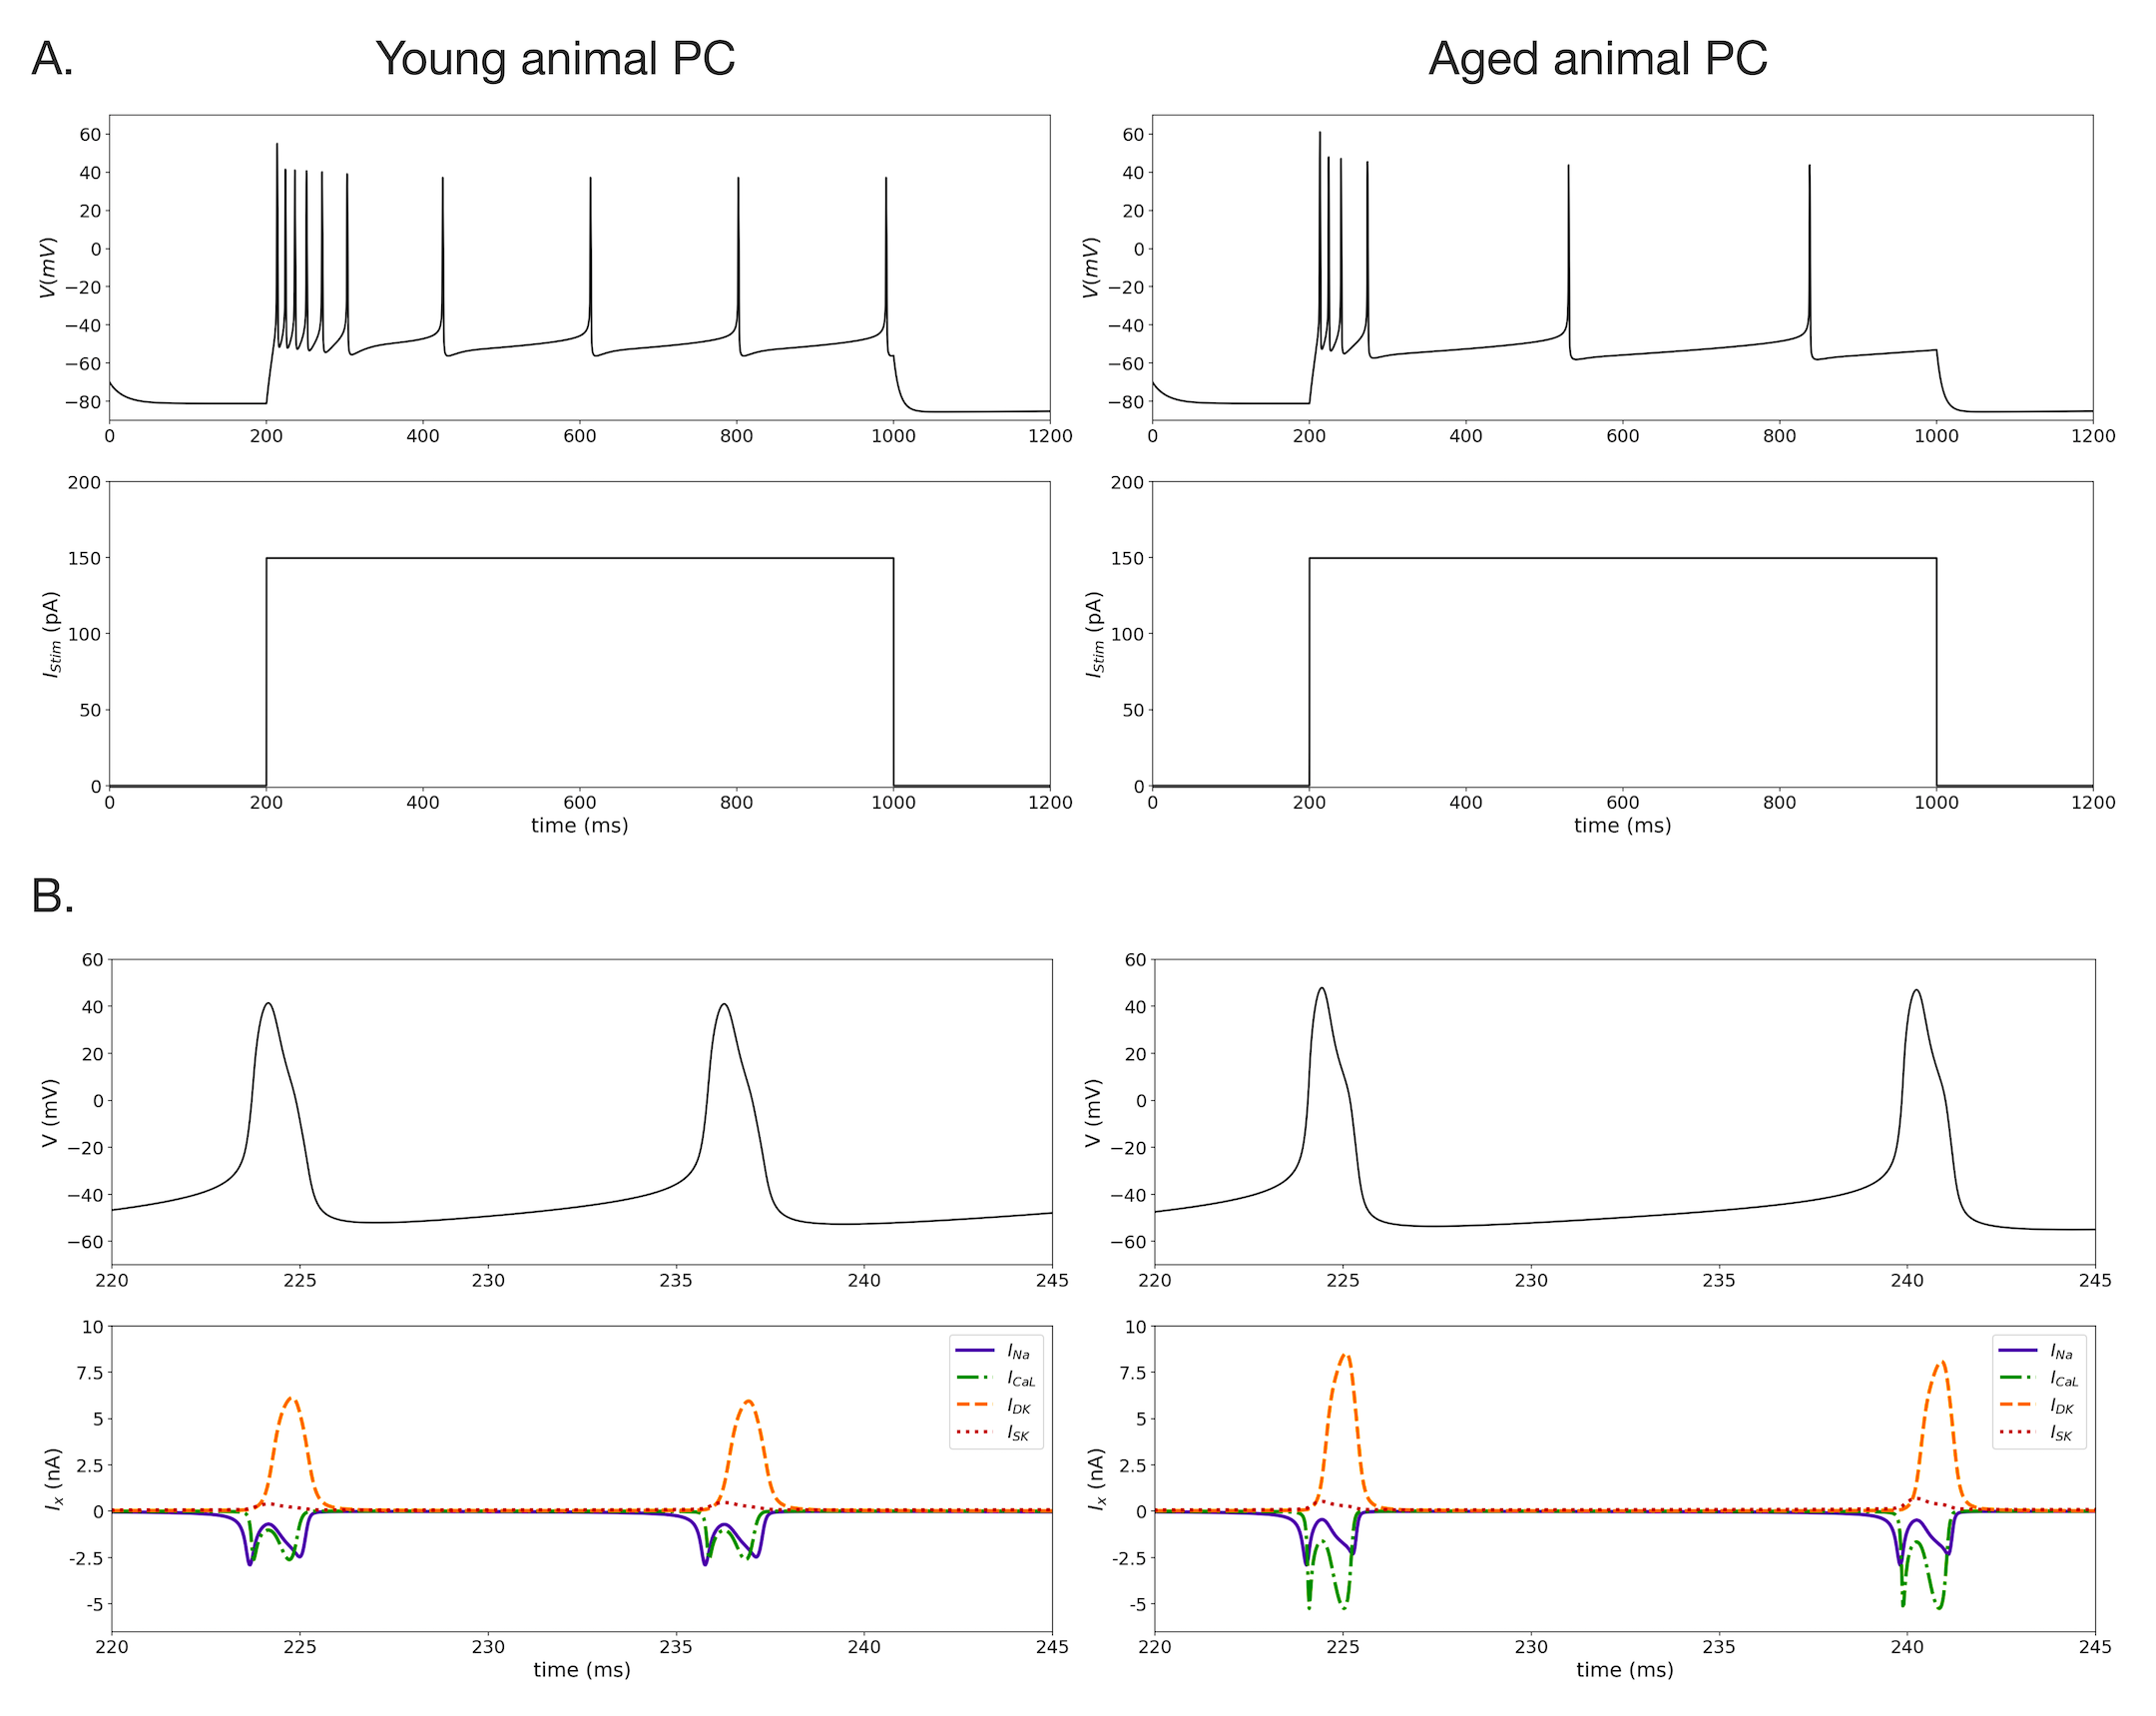
\includegraphics[width=0.99\textwidth]{figures/fig1.png} 
    \caption{Responses of yPC (left column) and aPC (right column)  models to an 800 ms 150 pA square pulse current injection. \textbf{A.} Top row shows the voltage responses of each cell to the stimulus shown in the second row. \textbf{B.} Zoom-in on two APs fired early in the response to better visualize their time course and amplitude, while below shows the amplitude and dynamics of the corresponding ionic currents. Parameters for yPC: $a_{NaT}$ = 1000, $a_{CaL}$ = 25, $a_{DK}$ = 8000, $a_{SK}$ = 1400, $r_{w}$ = 1.0, $r_{c}$ = 1e$^{-3}$, and $k_{c}$=3e$^{-6}$. All parameters for aPC the same except $a_{CaL}$=50. Units for all parameters can be found in Table \ref{tab:params}.}
    \label{fig:adaptation}
\end{figure}

Studies show that adaptation is more pronounced in aged than in young animals, leading to a shorter initial period of fast spiking, followed by fewer spikes or even complete cessation of firing \citep{disterhoft1996calcium,gant2006early,moyer1992nimodipine,tombaugh2005slow}. Stronger adaptation in PCs from aged animals may be relevant to circuit function, as it is correlated with learning impairment \cite{disterhoft1996calcium,tombaugh2005slow}. To compare the yPC and aPC models, all parameters were fixed except for the maximum amplitude of the L-type {\Ca} current, which was set to produce currents of $\sim$2-3~nA (young) or $\sim$5-6~nA (old), based on recordings \citep{campbell1996aging}. Increased {\Ca} channel density in the aPC model causes the number of spikes fired in the first $\sim$100 ms after stimulus onset to decrease from 6 to 4 spikes, and further slows firing for the remaining period of current injection (Fig.~\ref{fig:adaptation}A, right column). These results are similar to those found in recordings of CA1 PCs in young and old rabbits \citep{moyer1992nimodipine}.

Comparing the ionic currents produced in each PC model during individual APs (Fig.~\ref{fig:adaptation}B), we see that the {\Na} currents are equivalent in the two cells but the {\Ca} current in the aPC is approximately double that in the yPC, as expected with our parameter settings. Interestingly, despite setting the DK channel amplitude to be the same in the two cells, $I_{DK}$ was larger in the aPC by $\sim$2 nA. This increased $I_{DK}$ appears to be a consequence of the larger depolarization produced in the aPC model due to increased {\Ca} influx. The APs in the aPC are a few millivolts larger than those in the yPC, which increases the driving force for {\K} entry. However, increased $I_{DK}$ is not responsible for the stronger adaptation in the aPC, as this current decreases rather than increases as firing proceeds. Furthermore, scaling $I_{DK}$ back down in the aPC to compensate does not recover the firing pattern seen in yPCs. These results are not shown here, but can be confirmed by running the corresponding simulations in our Jupyter notebook (found at \href{https://github.com/emckiernan/agingCA1}{github.com/emckiernan/agingCA1}).

Examining the voltage response and the {\Ca} and SK currents generated in the first 120 ms after stimulus onset reveals the mechanisms underlying the stronger adaptation in the aPC model (Fig. \ref{fig:adaptzoom}). The large {\Ca} current causes the aPC to fire soon after stimulus onset. However, over time, the larger increase in intracellular {\Ca} in turn produces a larger SK current, which slows firing to a greater extent in the aPC. While the first two spikes occur nearly simultaneously in the aPC and yPC, by the third spike the aPC falls behind and the yPC spikes sooner. By the fourth spike, activity in the aPC is significantly delayed with respect to the yPC. The aPC fails to spike again in this time period, while the yPC fires again. Closer inspection of the voltage traces, especially following the fourth aPC spike, shows a prolonged AHP that prevents the cell from firing.

\begin{figure}[h!]
\centering
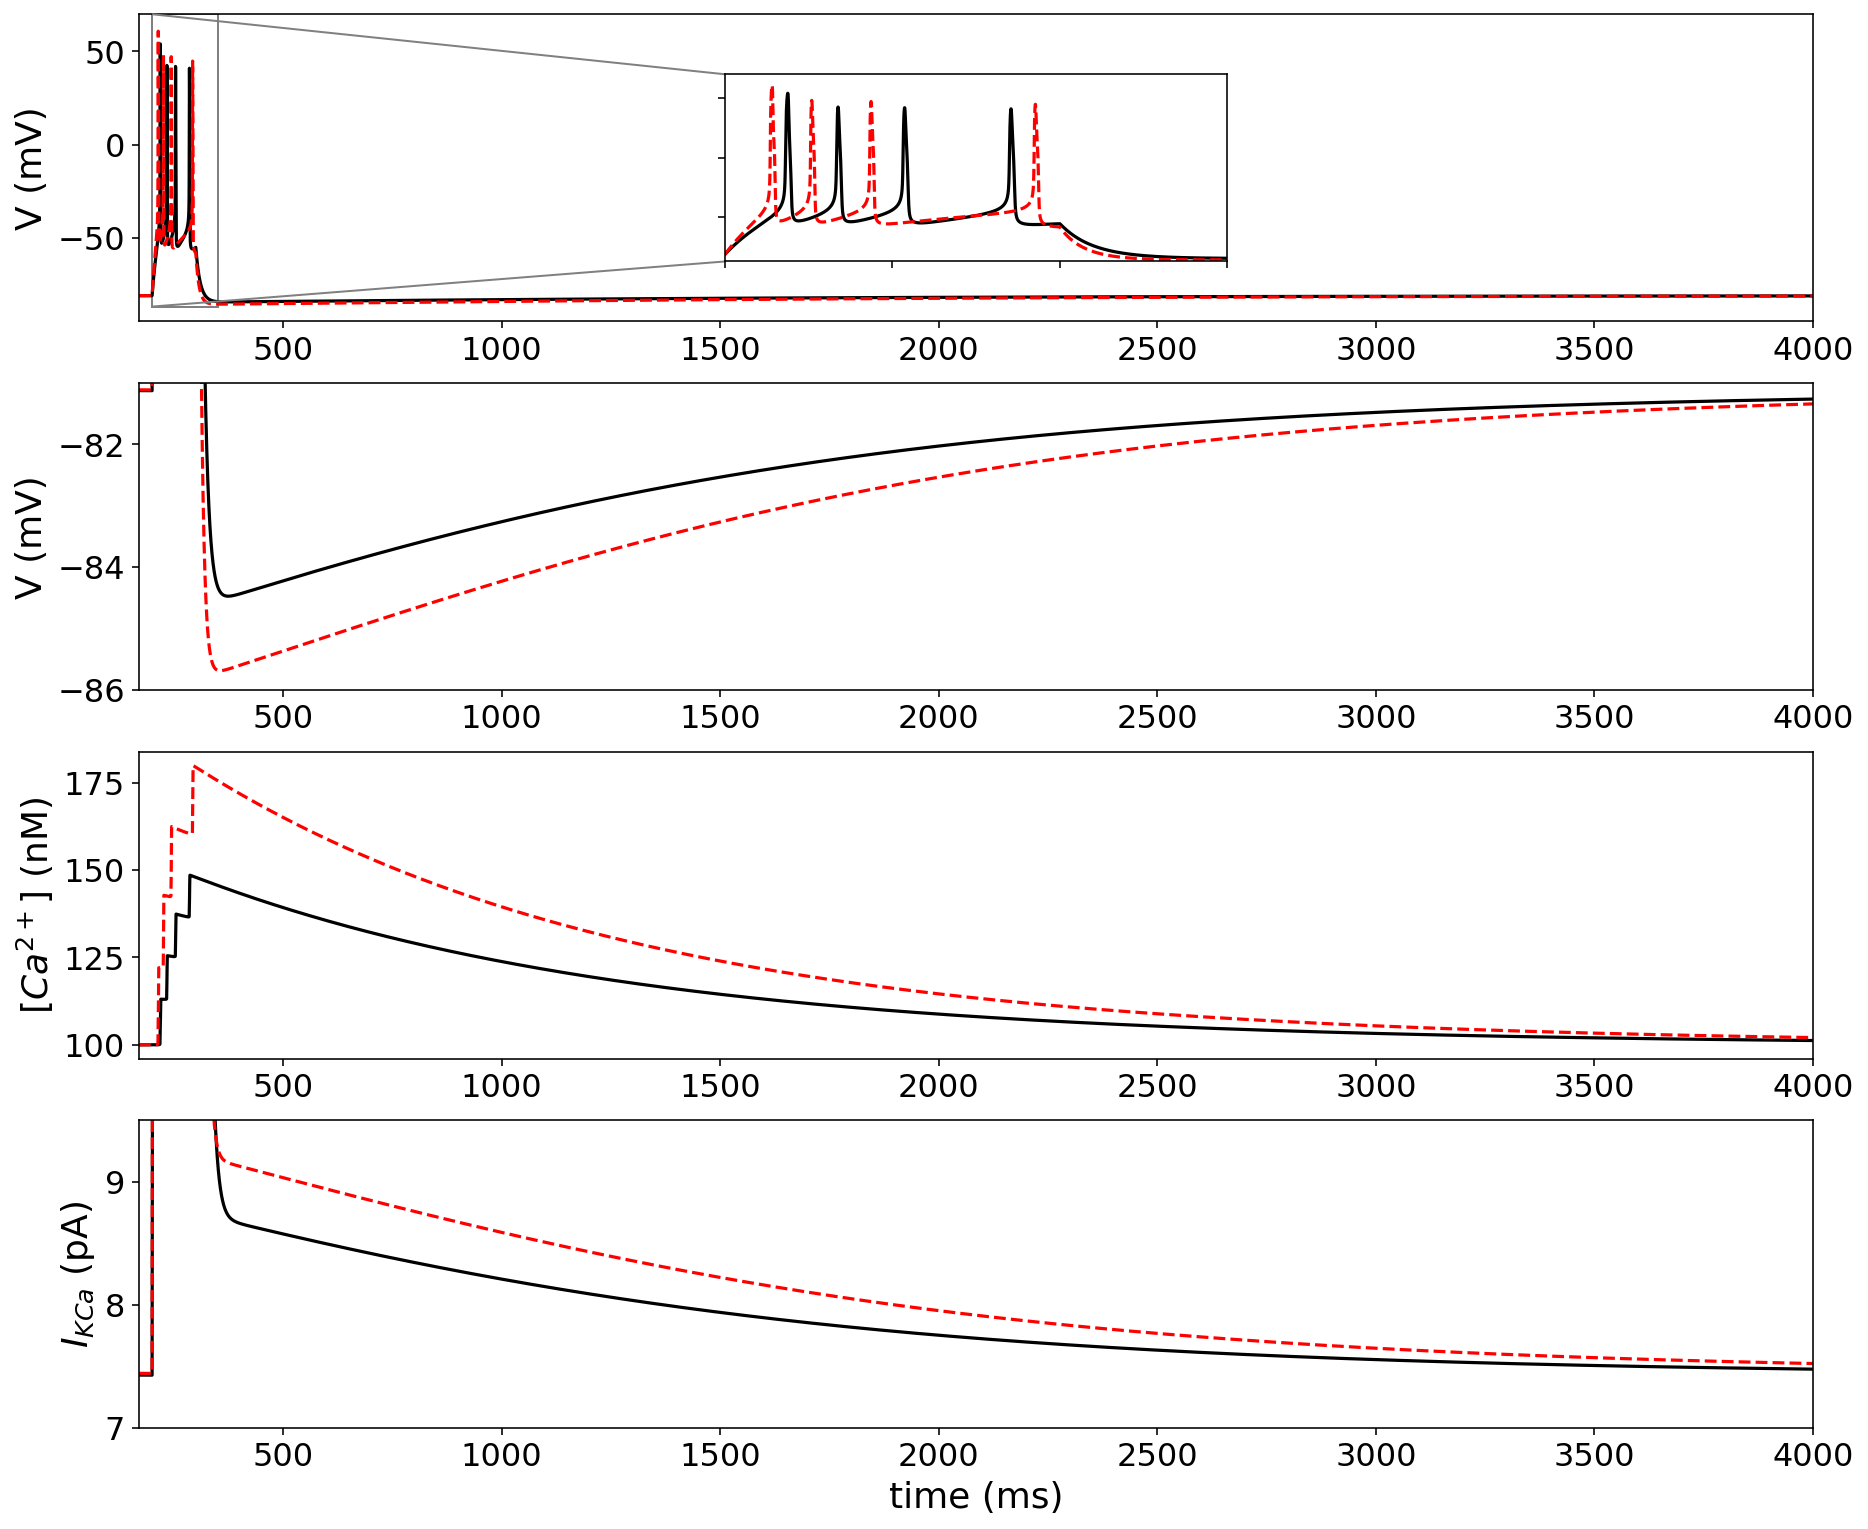
\includegraphics[width=0.9\textwidth]{figures/fig2.png}
\caption{Spike frequency adaptation in the yPC (solid black traces) versus aPC (dashed red traces) models. First 120 ms of voltage responses (top panel) shown in Fig. \ref{fig:adaptation}. Corresponding {\Ca} currents, intracellular {\Ca} concentration, and SK currents for each cell can be seen in the second, third, and fourth rows, respectively.}
\label{fig:adaptzoom}
\end{figure}

\subsection{Modeling age-related changes in AHPs}

AHP generation has been studied in CA1 PCs \citep{storm1989after,storm1990potassium,gu2005kv7}, particularly in the context of aging and excitability \cite{bodhinathan2010redox,blalock2010effects,disterhoft1996calcium,gant2006early,gant2009action,kaczorowski2009memory,matthews2009fast,power2002age,moyer1992nimodipine}. To induce AHPs, we kept the same parameters as in the previous simulations. We then stimulated model neurons with a 100 ms square pulse of sufficient amplitude to generate a burst of 4 APs (Fig. \ref{fig:AHP}). The AHPs produced under these conditions in the yPC model had a peak amplitude of $\sim$4 mV, similar to recordings \citep{kaczorowski2007stability,matthews2009fast,power2002age}.

The aPC model required more current than the yPC model to fire the same number of spikes (112 vs. 142 pA), suggesting that the aPC model is less excitable. However, the aPC fires earlier than the yPC due to its increased {\Ca} current (Fig. \ref{fig:AHP}, top panel inset). The aPC generates an AHP  $\sim$1-2 mV larger than seen in the yPC (Fig. \ref{fig:AHP}, second panel), similar to the magnitude of the difference observed in recordings \citep{moyer1992nimodipine,blalock2010effects,gant2006early,power2002age}. In the model, this larger AHP is due to an increased accumulation of {\Ca} in the aPC, which in turn produces a larger SK current (Fig. \ref{fig:AHP}, third and fourth panels).

\begin{figure}[h!]
\centering
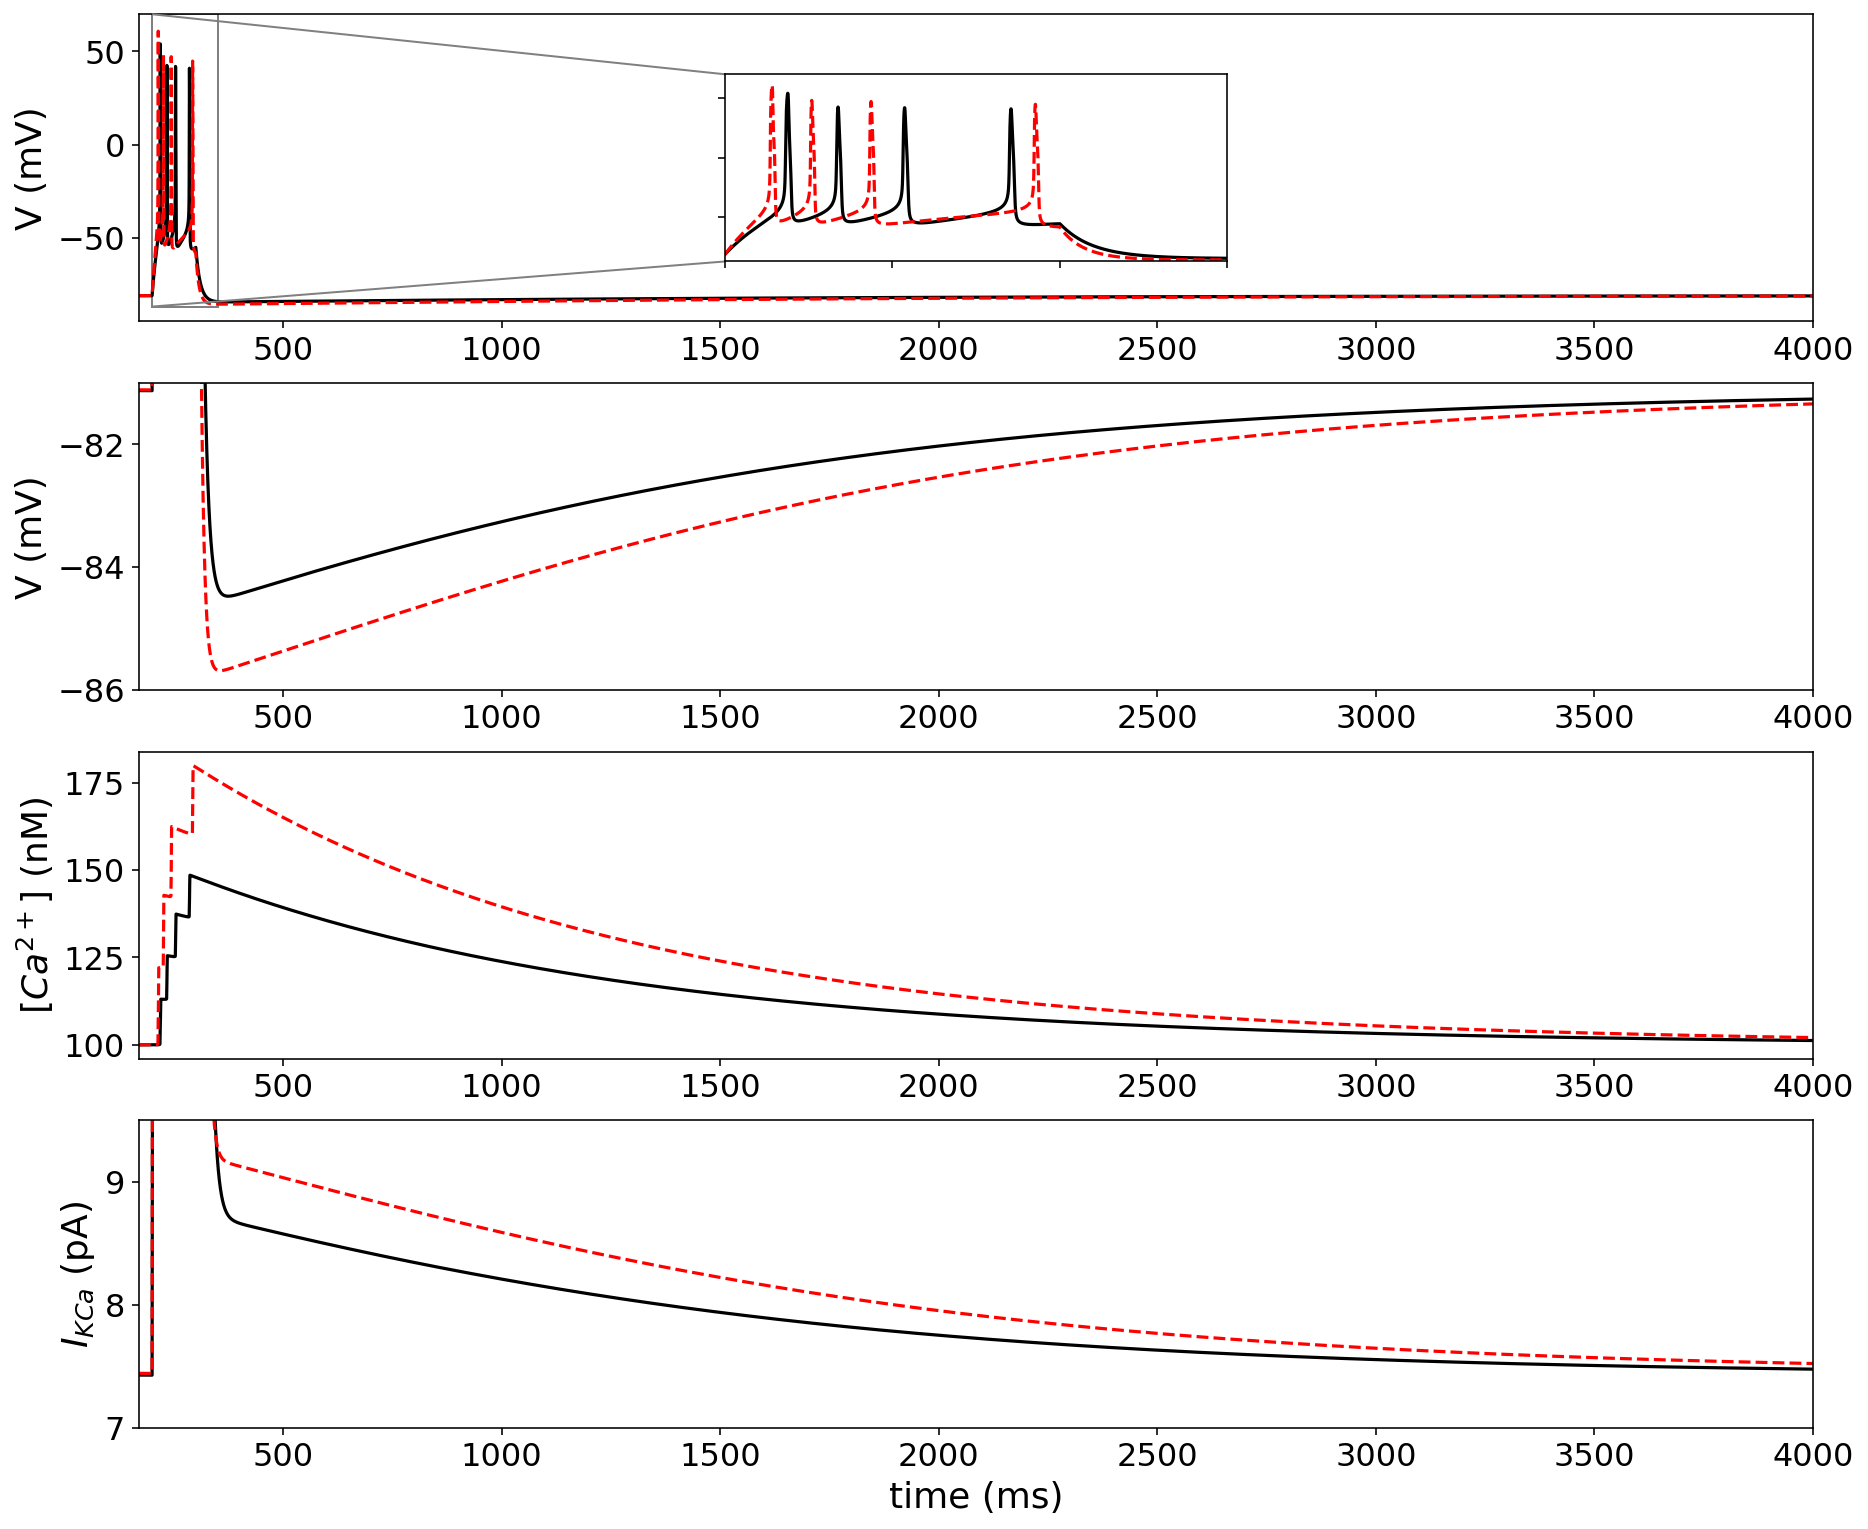
\includegraphics[width=0.85\textwidth]{figures/fig3.png}
\caption{Responses of the yPC (solid black traces) and aPC (dashed red traces) models to 100 ms pulse (top panel). Current amplitude adjusted to produce 4 spikes in each cell (yPC: 112 pA; aPC: 142 pA). Inset zooms in to see the temporal relationship of spiking in the two cells. Second panel zooms in to better show the amplitude and time course of the AHP. The intracellular {\Ca} concentration and SK currents for each cell can be seen in the third and fourth panels, respectively. Same parameters as previously. }
\label{fig:AHP}
\end{figure}

\subsection{Modeling age-related changes in burst firing}

\subsubsection{Bursting in response to stimulation}

Some CA1 PCs fire bursts instead of trains of individual spikes, \citep{azouz1996ionic,jensen1994variant,su2001extracellular,golomb2006contribution}, especially in certain developmental periods \citep{chen2005transitional}. Burst firing can be generated in the model with several different parameter combinations. For the following simulations, we increased the amplitude of the {\Na} current, decreased the amplitude of the DK current and increased its activation time constant, increased the amplitude of the SK current, and made changes to the {\Ca} handling, all within physiological limits. Under this parameter regime, model PCs are silent at rest but burst if stimulated (Fig. \ref{fig:burstStims}).

\begin{figure}[h!]
\centering
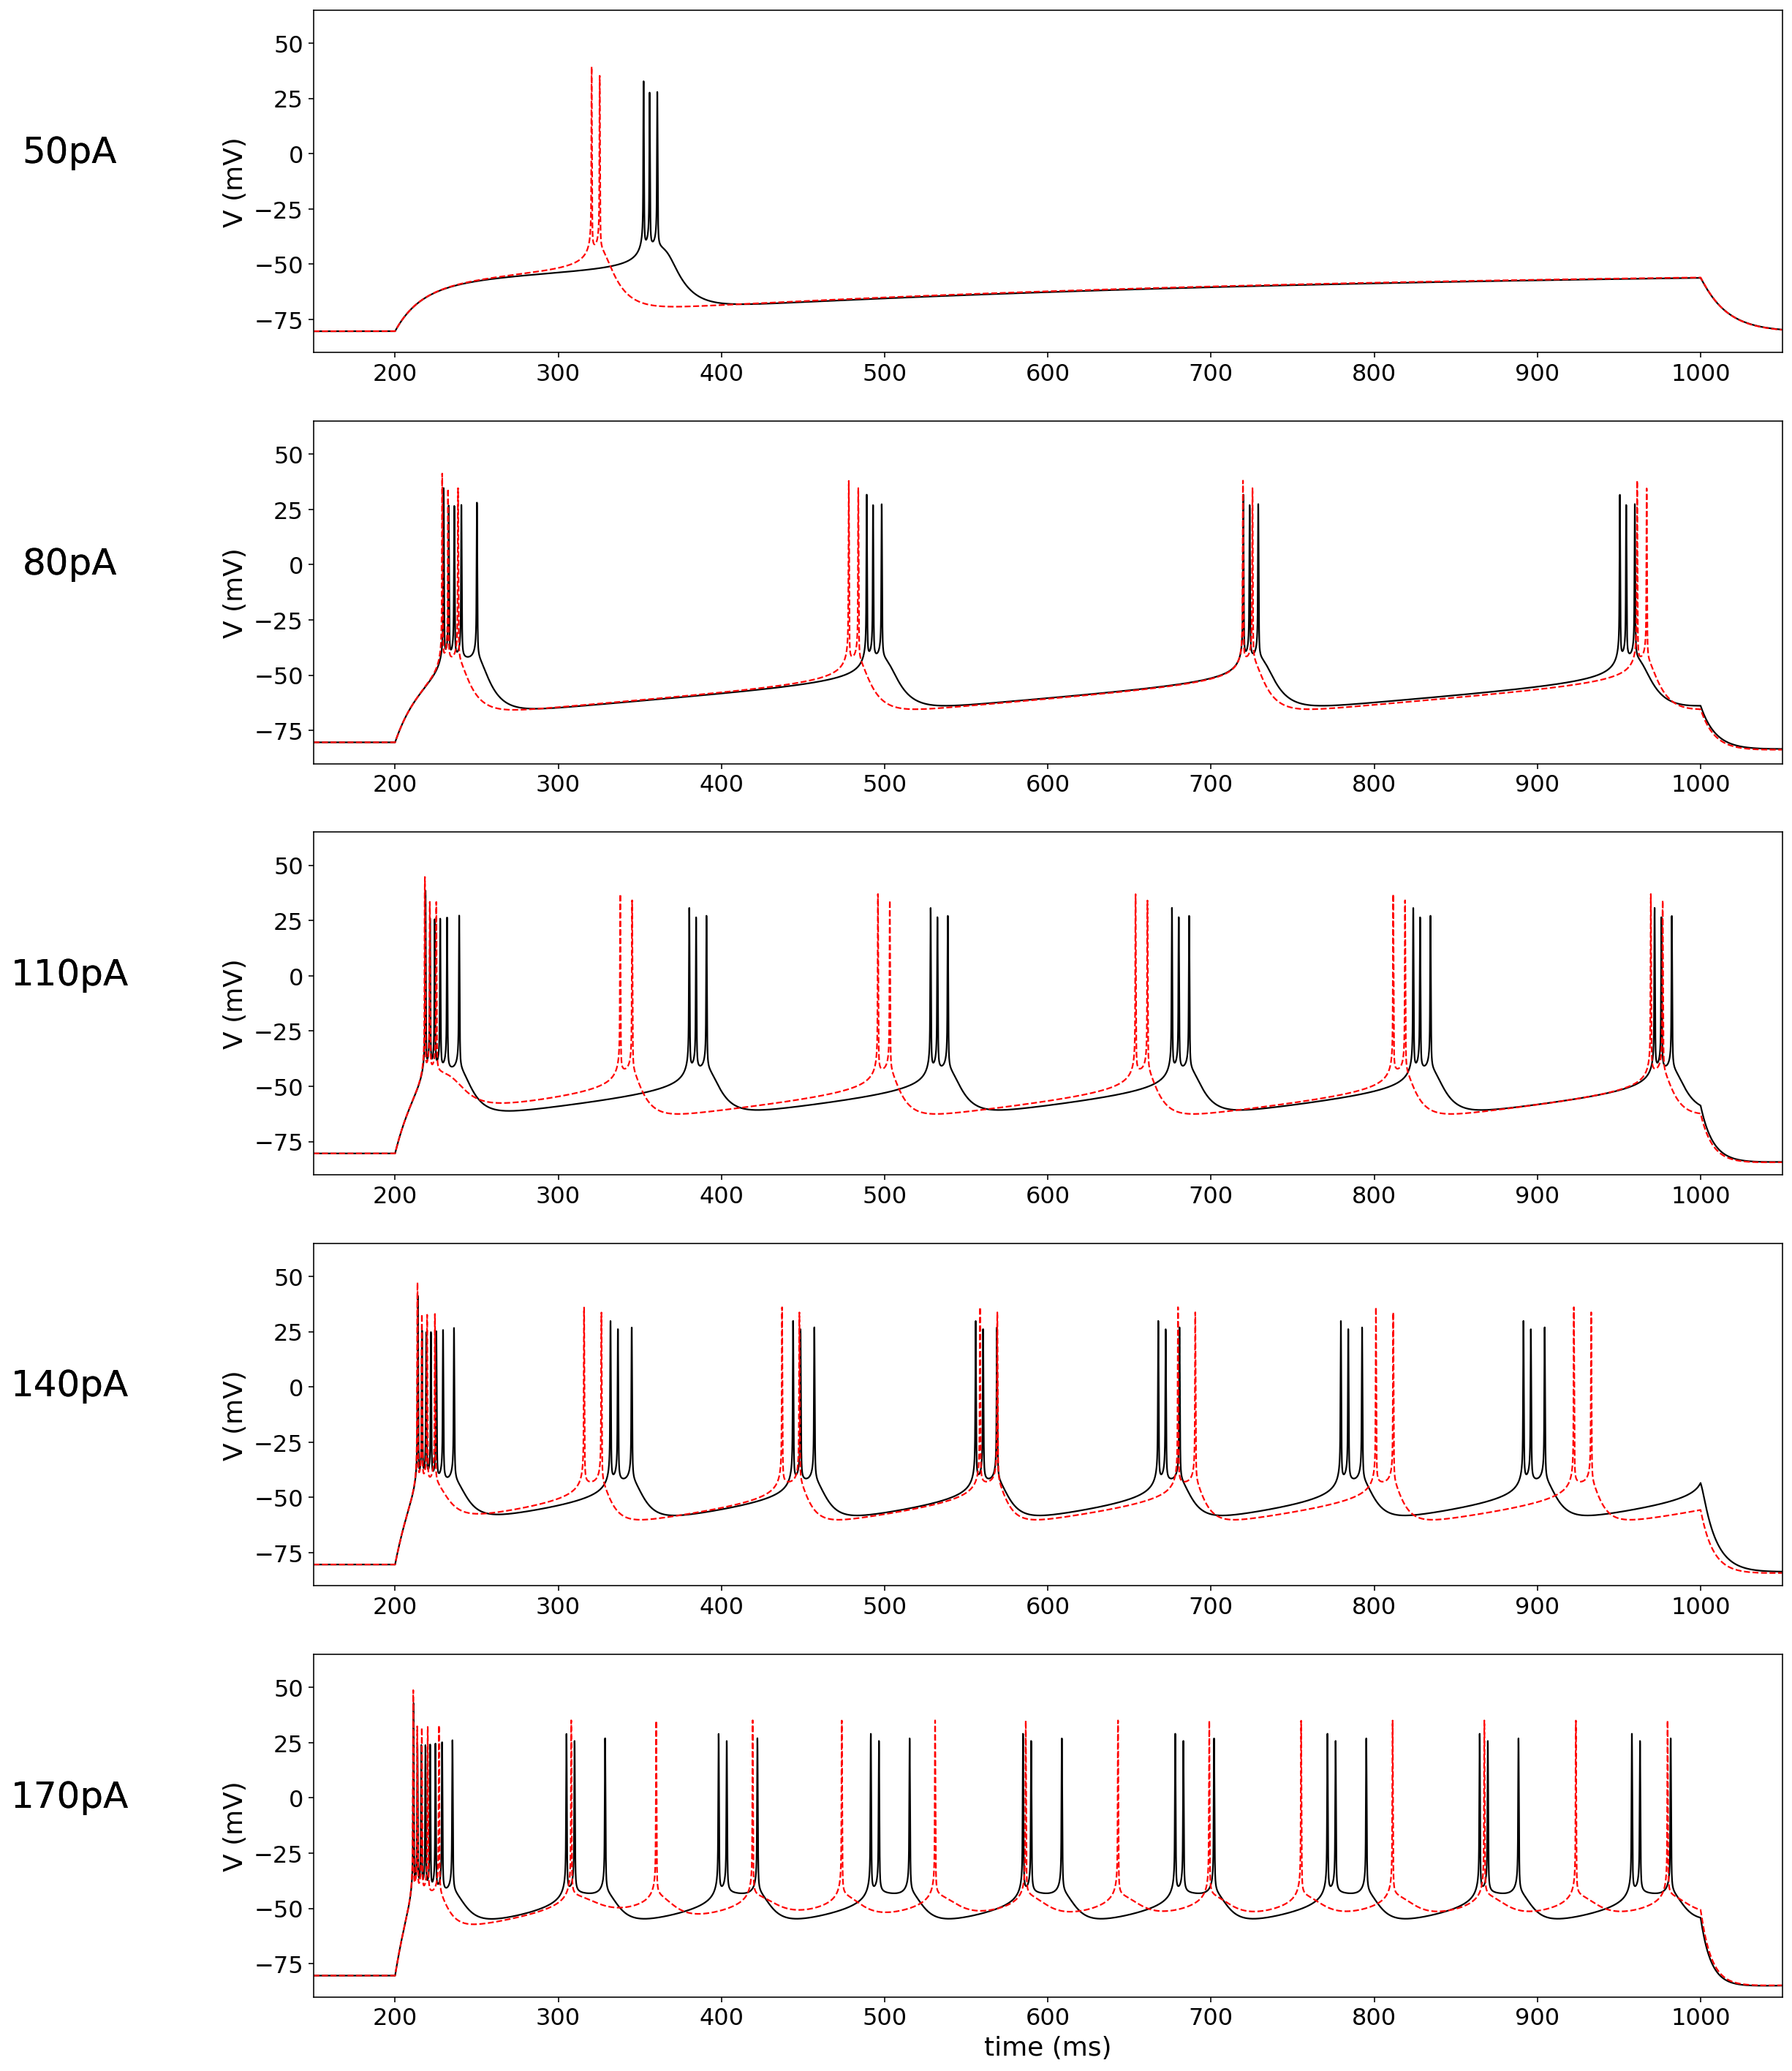
\includegraphics[width=0.95\textwidth]{figures/fig4.png}
\caption{Bursting in the yPC (solid black traces) and aPC (dashed red traces) models in response to 800 ms current injections of varying stimulus amplitudes (indicated to the left of each panel). Parameters for yPC: $a_{NaT}$ = 1300, $a_{CaL}$ = 25, $a_{DK}$ = 6000.0, $a_{SK}$ = 1600, $r_{w}$ = 1.8, $r_{c}$ = 5e$^{-3}$, $k_{c}$ = 6e$^{-6}$. All parameters for aPC the same except $a_{CaL}$ = 50.}
\label{fig:burstStims}
\end{figure}

To explore the effects of aging on bursting, we fixed all parameters except for the maximum {\Ca} current amplitude, as in previous simulations. We then stimulated the two model PCs with a series of square pulse current injections ranging from 50 to 170 pA in steps of 30 pA to compare their responses. As mentioned previously, the larger {\Ca} current in the aPC model causes it to fire either sooner or nearly simultaneously with the yPC shortly after stimulus onset in all simulations. However, the relative timing of the two PCs' firing after the first burst depends on the stimulus amplitude (Fig. \ref{fig:burstStims}).

At 50 pA, the aPC model bursts sooner but fires fewer spikes per burst than the yPC model. At 80 pA, the initial bursts of the two PCs are nearly coincident, and the cells continue to fire almost at the same time, with only slight differences in burst times. At 110 pA, the two PCs again fire nearly simultaneously at the onset. However, because the aPC fires fewer spikes per burst, it is able to recover sooner and burst before the yPC for several cycles. It is only towards the end of the stimulus that the larger AHP in the aPC eventually brings it into sync again with the yPC. At 140 pA, both PCs show stronger adaptation, with the time between the spikes in their bursts increasing. The two PCs maintain similar burst timing until the last few cycles, when the aPC falls behind the yPC. Finally, at 170 pA, the interspike interval in the aPC becomes so large that it spikes tonically rather than bursting, while the yPC continues to fire what could be seen as bursts, though with a delayed third spike in each. Depending on what we consider the relevant electrical event -- the single spike or the burst -- the aPC shows an increased number of events relative to the yPC, but the normal bursting pattern is lost. 

\subsubsection{Spontaneous bursting}
A small percentage of CA1 PCs fire spontaneous bursts in the absence of stimulation \citep{jensen1994variant,jensen1996spike,su2001extracellular}. To generate spontaneous bursting in model neurons, we increased the amplitude of both the {\Na} and DK currents, decreased the time constant of activation for the DK current, and decreased the amplitude of the SK current. Under this parameter regime, the yPC model fires spontaneous bursts at a frequency of $\sim$1 Hz with 3 spikes per burst (Fig. \ref{fig:spontBurst}), similar to recordings \citep{golomb2006contribution}.

\begin{figure}[h!]
\centering
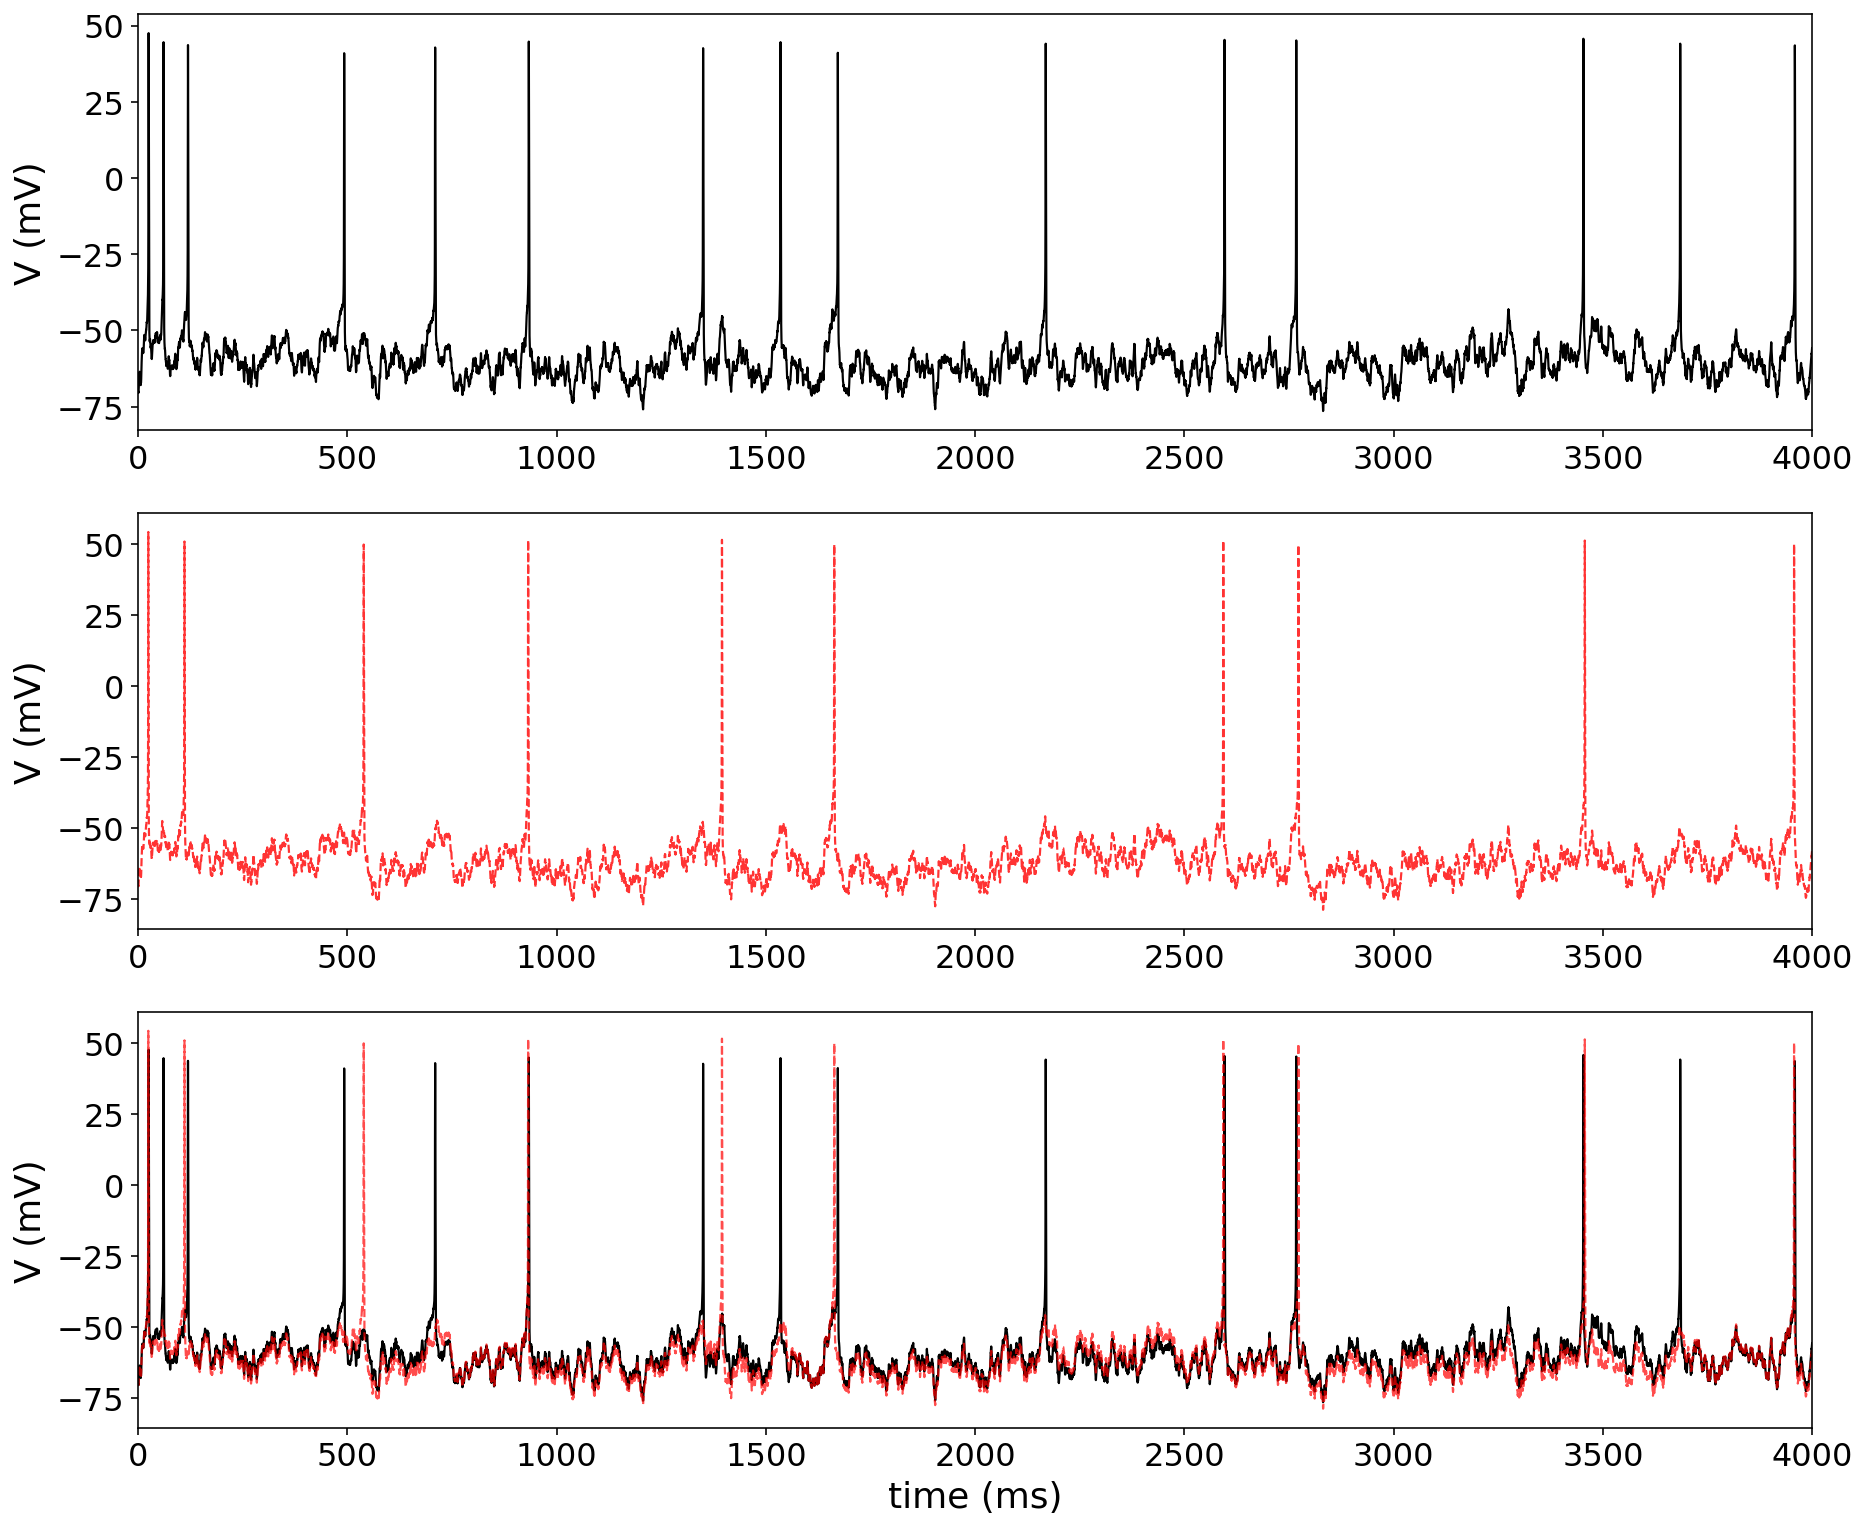
\includegraphics[width=0.8\textwidth]{figures/fig5.png}
\caption{Spontaneous bursting in the yPC model. Parameters: $a_{NaT}$ = 2300, $a_{CaL}$ = 25, $A_{DK}$ = 7000, $a_{SK}$ = 300, $r_{w}$ = 1.1, $r_{c}$ = 5e$^{-2}$, $k_{c}$ = 6e$^{-6}$, $I_{F}$ = 0.0.}
\label{fig:spontBurst}
\end{figure}

Increasing the {\Ca} channel density to simulate aging, as previously, change the spontaneous firing pattern (Fig. \ref{fig:burstingAging}). Additional interesting effects can be seen if we vary the DK current amplitude within the range previously used for simulations, 6000-8000 pA (6-8 nA) in steps of 500 pA. At the highest level of DK current amplitude (8 nA), the yPC continues to burst spontaneously, as seen in Fig. \ref{fig:spontBurst}, at a frequency of $\sim$1Hz but with only 2 spikes per burst. The aPC, on the other hand does not burst, but rather spikes tonically at a frequency of $\sim$2Hz. When the DK current amplitude is reduced (7.5 nA), the yPC continues to burst, now with 3 spikes per burst, while the aPC continues to spike tonically. 

\begin{figure}[h!]
\centering
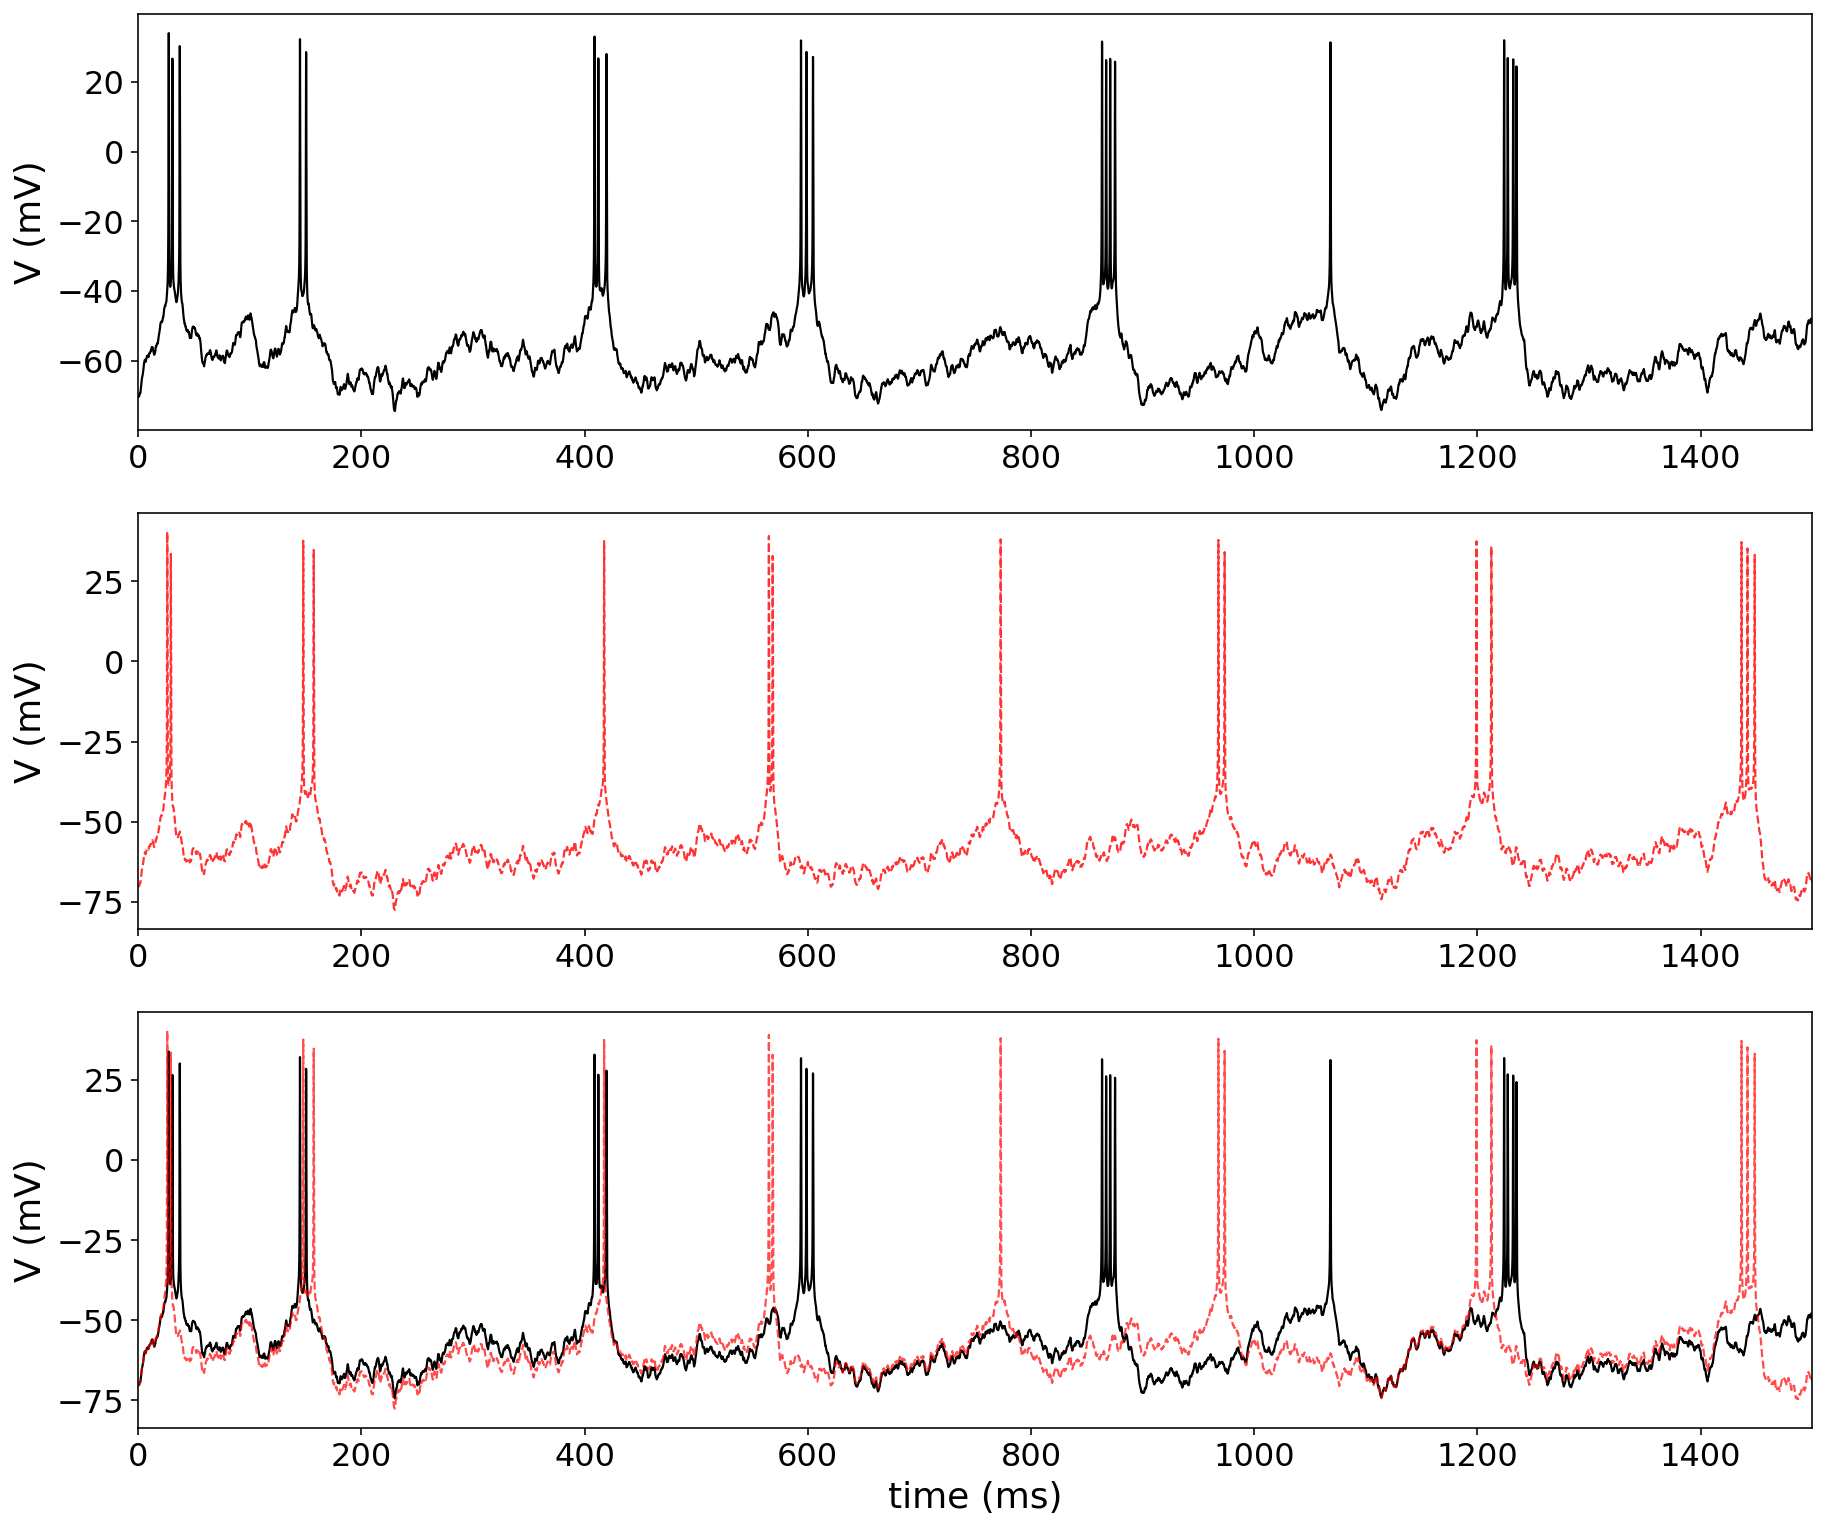
\includegraphics[width=0.95\textwidth]{figures/fig6.png}
\caption{Comparison of spontaneous electrical activity in the yPC (solid black traces) and aPC (dashed red traces) for different levels of DK current amplitude. $a_{DK}$ decreasing from 8000 to 6000 pA (8 to 6 nA) in steps of 500 pA, as indicated. Other parameters for yPC the same as in Fig. \ref{fig:spontBurst}. All parameters for aPC the same except $a_{CaL}$ = 50.}
\label{fig:burstingAging}
\end{figure}

Reducing the DK amplitude further (7 nA), now causes both PCs to burst spontaneously, though the aPC fires only 2 versus 3 spikes per burst. While the {\Ca} current is larger for the aPC model, the maximum accumulation of {\Ca} is only $\sim$10-15 nM more than in the yPC. There is a larger SK current in aPC due to the increased {\Ca}, but again, because the yPC fires an additional time, the two cells end up reaching nearly the same maximum current amplitude (only a $\sim$15 pA difference). In other words, the `brake' on the two cells is almost equal, and the larger {\Ca} influx in the aPC model then means that it can burst at a slightly higher frequency. 

Decreasing the DK amplitude still further (6.5 nA), removes some of the `brake' on the yPC and causes it to increase the number of spikes per burst to 5, while the aPC remains at 2 spikes per burst. This increased spiking causes the {\Ca} accumulation per burst to now be larger in the yPC, despite its lower amplitude setting, relative to the aPC. In turn, the yPC experiences a larger SK current and bursts one less time than the aPC. Finally, reducing the DK amplitude to its lowest level (6.0 nA), removes the remaining `brake' on the yPC and causes it to spike at high frequency and then quickly become block depolarized. The aPC, on the other hand, retains the normal spontaneous burstng pattern, now with 3 spikes per burst. These results illustrate the importance of the balance between the different ionic currents, and have interesting implications for our thinking regarding aged PC excitability (see Discussion).

\subsection{Responses to local field potential forcing}
Square pulse stimulation is useful and crucial for examining the timing of neural responses and also to calibrate the model so that the different currents yield responses like those observed experimentally. However, square pulse stimulation is not a physiologically realistic stimulus. Instead, to simulate local field potential (LFP) forcing onto CA1 PCs, we use an Ornstein-Uhlenbeck stochastic process \citep{rudolph2004method,destexhe2004novel}, as in Eq. \ref{eq:OU}. We began by stimulating model PCs with parameters set to produce an adaptive firing pattern, as in Section \ref{sec:adaptation}. In the yPC model, LFP forcing produced repetitive, irregular firing at a frequency of $\sim$3Hz on average (Fig. \ref{fig:LFPadaptive}, top panel). This firing pattern and frequency is similar to recordings of spontaneous firing in CA1 PCs \citep{manseau2017tuning,yang2017dl}, particularly in response to specific brain rhythms recorded in the surrounding field \citep{bland2002relationship,bland2005heterogeneity,huh2016excitatory}.

The aPC model with increased {\Ca} channel expression show a similar irregular firing pattern, but with a slower frequency  (Fig. \ref{fig:LFPadaptive}, second panel; also compare overlap in third panel). In a time window of 4 seconds, the yPC model fires 14 times, while the aPC fires only 9 times. In fact, the simulation shows several time points when the two cells fire almost simultaneously and then the yPC model fires again while the aPC fails to do so. This apparent `spike failure' has been observed in recordings of PCs from aged animals \citep{gant2009action}. 
\begin{figure}[h!]
\centering
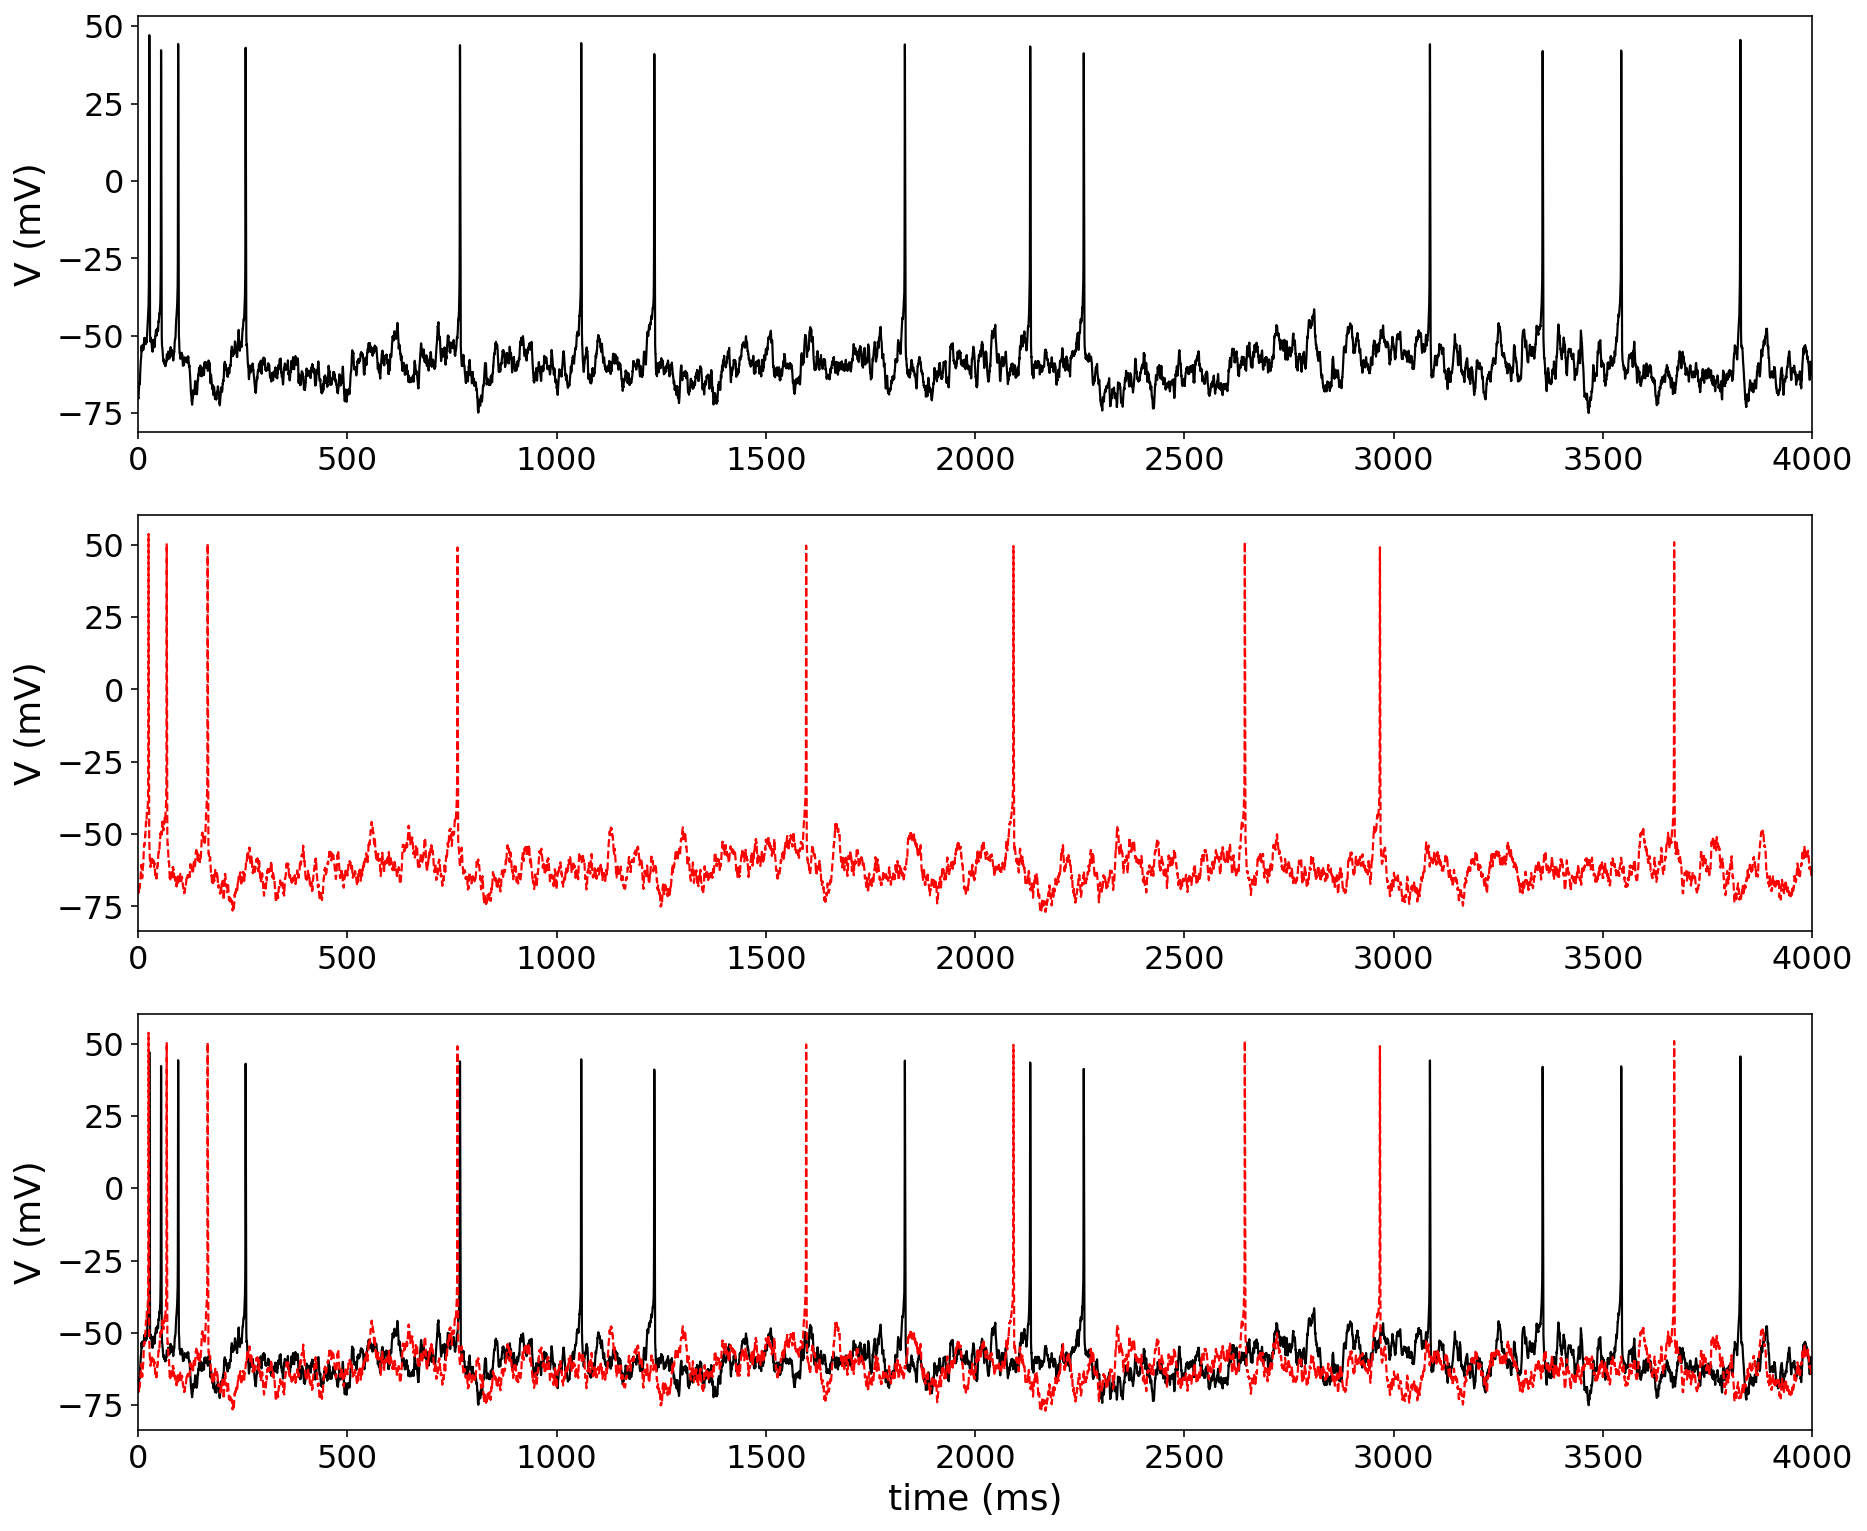
\includegraphics[width=0.9\textwidth]{figures/fig7.png}
\caption{Responses of yPC (solid black traces) and aPC (dashed red traces) models to LFP forcing while in adaptive firing mode. Top panel shows just the yPC response, the second panel shows the aPC response, and the third panel shows the overlap of the two traces. Parameters for yPC and aPC models same as in Fig.~\ref{fig:adaptation}. LFP parameters: $\mu_{F}$=50.0 pA, $\sigma_{F}$=25.0 pA, $\tau_{F}$=1/2.0 for both models.}
\label{fig:LFPadaptive}
\end{figure}

Next, we set the parameters to produce conditional bursting, as previously.\footnote{We also stimulated model PCs with LFP forcing when parameters were set to produce spontaneous bursting. This result is not shown here but can be explored in our Jupyter notebook (found at \href{https://github.com/emckiernan/agingCA1}{github.com/emckiernan/agingCA1}).} Under these conditions, LFP forcing in the yPC model produced irregular burst firing at a frequency of $\sim$4Hz (i.e., low end of theta frequency) with a variable number of spikes per burst (Fig. \ref{fig:LFPbursting}, top panel). This firing pattern is similar to spontaneous activity recorded in a subset of CA1 PCs known as phasic theta-ON cells, which preferentially burst during theta activity recorded from the surrounding field \citep{bland2002relationship,bland2005heterogeneity,colom1987state}. Increasing {\Ca} channel expression in the aPC model changes the firing pattern (Fig. \ref{fig:LFPbursting}, middle panel). In response to LFP forcing, the aPC still fires irregular bursts, but with fewer spikes per burst and a higher occurrence of 2-spike bursts than seen in the yPC. In addition, the aPC fires single APs amidst the bursts, which is not seen in the yPC under this parameter regime. Also, the timing of the bursts in the aPC model is altered relative to the yPC model (see third panel overlap). 

\begin{figure}[h!]
\centering
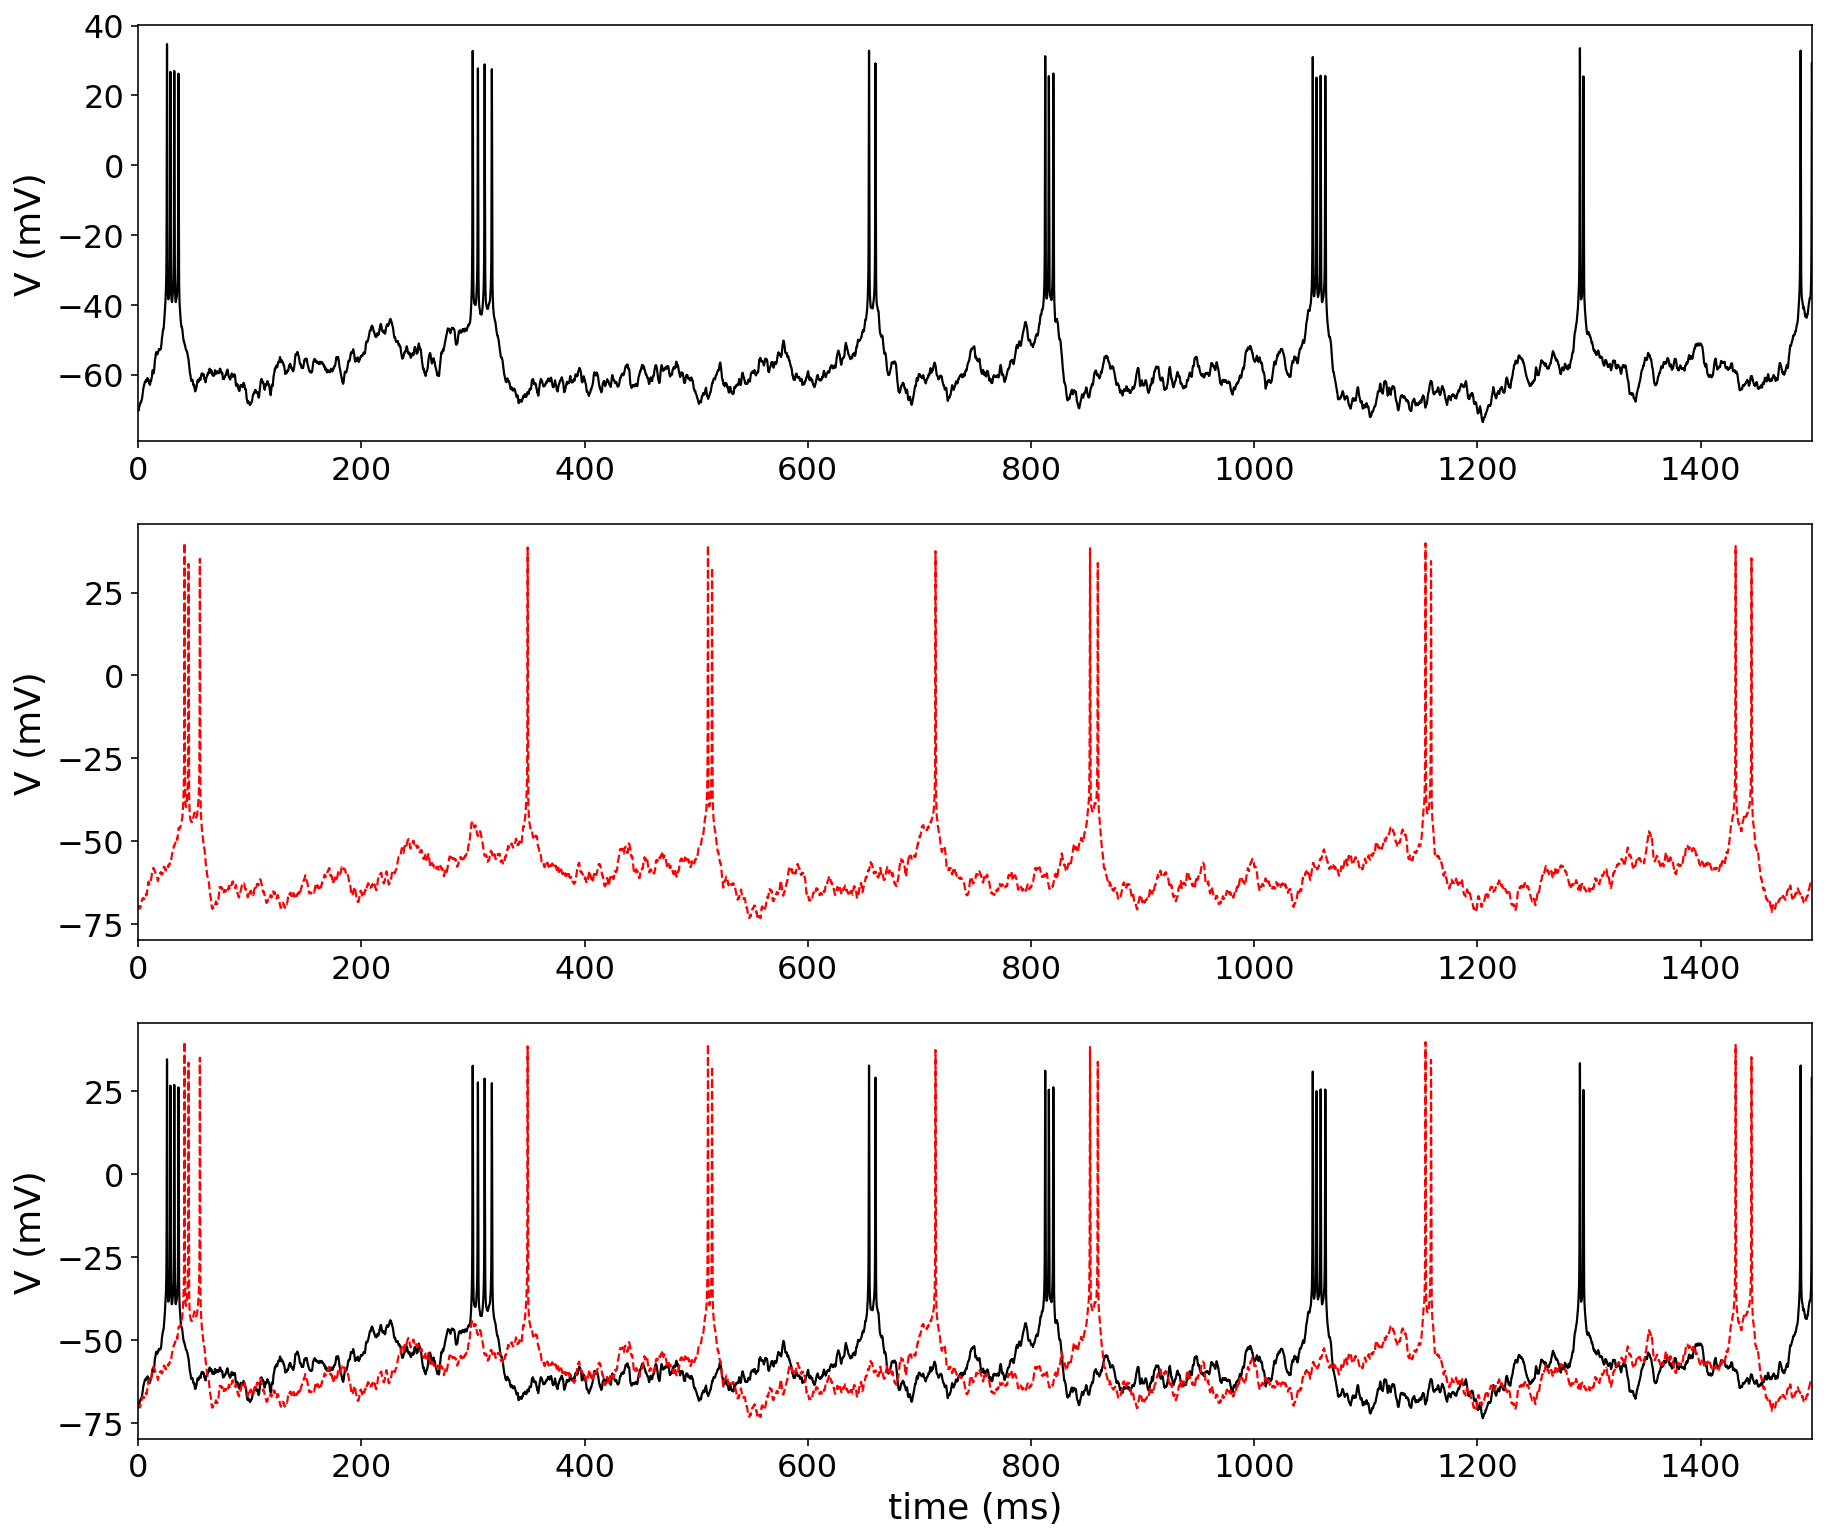
\includegraphics[width=0.9\textwidth]{figures/fig8.png}
\caption{Responses of the conditionally bursting yPC (solid black traces) and aPC (dashed red traces) models to LFP forcing. Top panel shows just the yPC model response, the second panel shows the aPC response, and the third panel shows the overlap of the two traces. Parameters for yPC and aPC models are the same as in Fig. \ref{fig:burstStims}. LFP parameters the same as in Fig. \ref{fig:LFPadaptive} except $\sigma_{F}$=20.0 pA.}
\label{fig:LFPbursting}
\end{figure}

\section{Discussion}

\subsection{Cellular heterogeneity}

Here we show that a three-dimensional, single-compartment model derived from first principles of thermodynamics is capable of reproducing the diversity of firing patterns recorded in CA1 PCs. Moving between the different adaptive and bursting firing patterns was achieved primarily by changes to the relative expression of ion channels in the model. While we did not systematically explore the full parameter space, future work could include bifurcation analysis to determine the boundaries for each firing pattern. 
The flexibility of the model could be useful for researchers looking to understand the effects of PC heterogeneity on network function. Geiller and colleagues \citep{geiller2017segregated} write, ``Until very recently, hippocampus models and theories were built on a view of homogenous population of principal cells'' (pg. 6). However, studies have shown that there is substantial heterogeneity in the firing patterns of CA1 PCs, especially during different development stages (for review, see \cite{mckiernan2017ca1}). Lee and colleagues \citep{lee2014parvalbumin} write, ``how the heterogeneous PCs integrate into the CA1 circuit remains unknown'' (pg. 1129). 

Experimentally, it is difficult to precisely quantify how many PCs in a given network are displaying a specific firing pattern, and even harder if not impossible to manipulate these percentages. Furthermore, cells can transition between firing patterns \citep{steriade1998dynamic}, meaning the percentages might fluctuate. With our minimal model, however, we could build small networks with different balances of adapting versus bursting PCs, for example, and explore how changing these balances affects network output.
We could also model the progression of aging in the network by varying the percentage of PCs which have altered {\Ca} channel density, or implement a whole spectrum of channel expression across the simulated network.

\subsection{Aging and {\Ca} channel expression}
Our model can also reproduce several changes in electrical activity observed in aged CA1 PCs, including larger AHPs \citep{kumar200217beta,kumar2007environmental,landfield1984prolonged,gant2009action,power2002age} and increased adaptation \citep{gant2006early,moyer1992nimodipine,tombaugh2005slow}. We show that an increase in the L-type {\Ca} current amplitude 
to a level similar to that recorded in aged PCs is sufficient to reproduce the characteristic changes in cellular excitability associated with aging. The L-type channel in our study was modeled after the Ca$_v$1.2 isoform based on work which implicates this channel as the primary contributor in rodent brain, responsible for $\sim$70-80\% of the L-type current \cite{hell1993identification,sinnegger2004isoform}. mRNA expression of \textit{Cacnac1C} (the gene encoding Ca$_v$1.2) is increased in aged mice and rats \cite{herman1998up,zanos2015sex}. Increases in plasma membrane expression \cite{nunez2014surface} and phosphorylation \cite{davare2003increased} of Ca$_v$1.2 channels, both of which could lead to an increase in the number of `functionally available' channels, have also been observed in aged rats. In addition, changes in \textit{Cacna1c}/Ca$_v$1.2 expression are correlated with memory impairments \cite{moosmang2005role,zanos2015sex}.

However, CA1 PCs also express the Ca$_v$1.3 isoform \cite{bowden2001somatic}, which is responsible for $\sim$20\% of the total L-type current \cite{hell1993identification,sinnegger2004isoform}. Studies have found both increased mRNA \cite{herman1998up} and protein \cite{veng2002regionally} expression of Ca$_v$1.3 in aged rats, and this increased expression is correlated with memory impairment \cite{veng2003age}. Knockout studies in mice indicate it is this isoform, and not Ca$_v$1.2, which contributes to slow AHP generation \citep{gamelli2011deletion}, possibly via activation of colocalized SK channels \cite{bowden2001somatic}. While experimental studies have been complicated by a lack of pharmacological agents which can isolate currents carried by the different isoforms, it would be relatively simple with our model to study the contributions of these two channels. The primary difference between the two is a shift in the activation curve of the Ca$_v$1.3 channel to more hyperpolarized values, relative to Ca$_v$1.2, with half-activation potentials of around -20mV versus +3mV, respectively \citep{xu2001neuronal}. In the model, changing the parameter $v_j$ in Eq. \ref{eq:gating} would allow us to represent the different isoforms to explore how changes in the expression of each during aging might affect PC excitability.  

Of course, there are many cellular changes apart from {\Ca} channel expression that occur during aging and could contribute to altered electrical activity in PCs. For example, several studies have implicated {\Ca} release from intracellular stores as an important contributor, particularly to larger AHPs in aged animals \citep{gant2006early,bodhinathan2010redox}
(for reviews see \citep{thibault2007expansion,toescu2010calcium}). We did not explore the role of intracellular {\Ca} stores in this study, nor many of the other cellular changes that surely contribute to the multifactorial process of aging. It is not our intention to suggest that altered {\Ca} channel expression is \textit{the} factor altering the excitability of PCs in aged animals; it may not even be the most important factor. We simply demonstrate that an increase in L-type {\Ca} channels is \textit{sufficient} to reproduce many of the changes in PC firing seen during aging. In addition, while some of the modeling results we report here may hold experimentally at the cellular level (i.e., \textit{in vitro} or \textit{in situ}), very different effects may be seen in the intact animal (i.e., \textit{in vivo}) where all neuronal, circuit-level interactions are preserved. It is known that the brain can compensate in a myriad of ways for changes in cellular excitability and gene expression \cite{grashow2010compensation,kim2017nonreciprocal}, and these compensatory mechanisms may work differently \textit{in vivo} versus \textit{in vitro} \cite{echegoyen2007homeostatic,morgan2019kv1}.

\subsection{Aging and excitability}
 Our simulations do show changes in the electrical activity of aged PCs, but do these changes represent decreased excitability? This question relates more broadly to how we think about excitability -- the term is rarely clearly defined or used in a standardized way. In some studies, excitability is used to refer to change in firing rate of a cell over the course of an injected current pulse, claiming that PCs with stronger adaptation are less excitable (e.g., \cite{moyer1992nimodipine,oh1999metrifonate}). In our simulations under the adaptive firing parameter regime, the aPC model did have stronger adaptation and fired fewer times during the stimulation period than the yPC model. However, under some circumstances, this stronger adaptation occurred only after the aPC model cell initially fired faster than the yPC model (see for example Fig. \ref{fig:AHP} inset). Should we consider this decreased excitability? 
 
 If what concerns us with excitability is the activity of the cell over a given time period, then the results under the bursting parameter regimes are even less clear. The aPC model always fired fewer APs per burst than the yPC, indicating something akin to stronger adaptation. However, if the `event' we are considering is instead the burst, there are conditions under which aPCs fired a greater number of bursts in a given time period than yPCs. How should we interpret these results with respect to excitability? To our knowledge, there are very few experimental studies to date that have compared burst firing in young versus aged animal PCs, perhaps because of the relatively low percentage of cells with this firing pattern in certain developmental periods \cite{chen2005transitional}. The only study of this type of which we are aware compared spontaneous burst firing in young versus aged animal PCs during rest and exploratory behavior \cite{smith2000effect}. Unfortunately, there are several factors that make it difficult to compare our results with theirs. First, their recordings were extracellular. As such, no bursts from individual PCs are shown in the paper to compare to our simulations, which reproduce intracellular firing patterns. Furthermore, the study focused on interspike intervals (ISIs), rather than the overall bursting pattern (e.g. number of bursts in a given period), which was our focus. Interestingly, Smith and colleagues \cite{smith2000effect} found that while ISIs were more left-skewed in aged animals when burst firing was recorded at rest, they found no difference between the age groups during behavior, suggesting that compensatory mechanisms work differently during behavior to adjust for changes in cellular excitability. Such compensatory mechanisms could be explored using our model, for example by adding simulated cholinergic input.     

Returning to the idea of excitability, other researchers use the term to refer to how easy it is to get a cell to fire in response to stimulation. For example, Daoudal and colleagues \cite{daoudal2003long} write, ``Excitability can be defined as a propensity of the neuron to generate, beyond a certain threshold, an output signal -- the action potential (AP) -- from a given input signal...'' (pg. 457). Similarly, Konstantinovi{\'c} and Filipovi{\'c} \cite{konstantinovic2019effects} write, ``Neuronal excitability can be defined...as the readiness of a nerve cell or a neural circuit to respond to a stimulus'' (pg. 234). In this context, excitability could be measured by the rheobase, or minimum current which generates firing in a neuron, as done in some studies of aging in CA1 (e.g., \cite{potier1993age}). However, `propensity' or `readiness' could also be interpreted as how quickly a cell fires after stimulus onset. In the AHP simulations, we saw that the aPC model  required 30 pA of additional current to fire the same number of spikes as for the yPC model. On the other hand, the aPC model often fired sooner than the yPC model and with larger amplitude APs in response to the same stimulus. These effects were a result of the increased {\Ca} channel density in aged cells -- the larger {\Ca} current depolarized the cells faster and caused them to fire sooner, but it also caused the {\Ca}-dependent SK current to be larger and consequently slowed firing. It is as if the aPCs were initially more excitable, but then `burned out' more quickly than the yPCs. 

Overall, we believe our results highlight the importance of moving away from vague, ill-defined terms like `excitability' in favor of clearer, more precise language that describes the effect of interest (e.g., PCs spiked faster, spiked sooner, etc.). We hope in a broader sense our study will encourage neuroscientists, and particularly aging researchers, to reevaluate how they think and write about excitability.

\section*{Funding} 
This work was supported by grants from the Natural Sciences and Engineering Research Council of Canada, as well as the Ontario Mental Health Foundation, awarded to DFM. This work was also supported by DGAPA-UNAM-PAPIIT IA209817 awarded to ECM; and by DGAPA-UNAM-PAPIIT IA208618, DGAPA-UNAM-PAPIIT IN228820, and DGAPA-UNAM-PAPIME PE114919 awarded to MAH-V.   
 
%\section*{Acknowledgments}  
 
% BIBLIOGRAPHY
\begin{small}
\bibliographystyle{unsrt}
\bibliography{pyrbib.bib}
\end{small}

\end{document}